\documentclass[11pt]{article}
\usepackage[utf8]{inputenc}

\title{}
\author{}
\date{}

% Packages
\usepackage{amsmath,amsfonts,amssymb,amsthm,rotating}
\usepackage{enumerate, enumitem}
\usepackage[left=3cm, right=3cm, top=3cm, bottom=2.5cm]{geometry}
\usepackage{mathrsfs, mathtools}
\usepackage[dvipsnames]{xcolor}
\usepackage{parskip}
\usepackage{graphicx}
\usepackage{float}
\usepackage[font=small,labelfont=bf]{caption}

\usepackage{cite}
\usepackage[numbers, authoryear, longnamesfirst, comma]{natbib}
\usepackage[nottoc]{tocbibind}
\usepackage{hyperref}
\renewcommand\bibname{Bibliography and References}

\interfootnotelinepenalty=10000

\setcitestyle{square}

%\usepackage[page, titletoc, title]{appendix}
%\renewcommand*\appendixpagename{Appendix}
%\renewcommand*\appendixtocname{Appendix}

\newcommand{\kolja}[1]{\textcolor{red}{#1}}

\usepackage{setspace}
\onehalfspacing

% Custom enviroments
\theoremstyle{definition}
\newtheorem{defn}{Definition}
\newtheorem{prop}{Proposition}
\newtheorem{lemma}{Lemma}
\newtheorem{thm}{Theorem}
\newtheorem{conj}{Conjecture}
\newtheorem{cor}{Corollary}
\newtheorem*{ex}{Example}
\newtheorem*{obs}{Observation}

% Front page
\begin{document}

\begin{titlepage}
\begin{center}
\begin{figure}[htb]
\begin{center}

\includegraphics[width=6cm]{matematiquesinformatica-pos-rgb.png}
\end{center}
\end{figure}
\vspace*{1cm}

\textbf{\LARGE GRAU DE MATEM\`{A}TIQUES } \\
\vspace*{.5cm}
\textbf{\LARGE Treball final de grau} \\
\vspace*{1.5cm}

\rule{16cm}{0.1mm} \\
\begin{Huge}
\textbf{Learning-Powered Computer-Assisted Counterexample Search.} \\
\end{Huge}
\vspace*{.5cm}
\begin{LARGE}
\textbf{Using Reinforcement Learning to Refute Spectral Graph Theory Conjectures.} \\
\end{LARGE}
\rule{16cm}{0.1mm} \\
\vspace{1cm}

\begin{flushright}
\textbf{\LARGE Autora: Laura Ventosa Andreu}
\vspace*{2cm}

\renewcommand{\arraystretch}{1.5}
\begin{tabular}{ll}
\textbf{\Large Director:} & \textbf{\Large Dr. Kolja Knauer} \\
\textbf{\Large Realitzat a:} & \textbf{\Large  Departament de Matem\`{a}tiques i Inform\`{a}tica} \\
\textbf{\Large Barcelona,} & \textbf{\Large \today }

\end{tabular}
\end{flushright}
\end{center}
\end{titlepage}

\setlength{\parindent}{0pt}

\newpage

\pagenumbering{roman}

\section*{Abstract}
This thesis explores the great potential of computer-assisted proofs in the advancement of mathematical knowledge, with a special focus on using computers to refute conjectures by finding counterexamples, sometimes a humanly impossible task. In recent years, mathematicians have become more aware that machine learning techniques can be extremely helpful for finding counterexamples to conjectures in a more efficient way than by using exhaustive search methods. In this thesis we do not only present the theoretical background behind some of these methods but also implement them to try to refute some graph theory conjectures.

\section*{Resum}
Aquest treball explora el gran potencial de les demostracions assistides per ordinador en l'avenç del coneixement matemàtic, centrant-se especialment en l'ús d'ordinadors per refutar conjectures trobant contraexemples, una tasca humanament impossible moltes vegades. En els darrers anys, investigadors i investigadores en matemàtiques han anat veient que l'aprenenatge automàtic, conegut com \textit{machine learning} en anglès, pot ser molt útil a l'hora de trobar contraexemples a conjectures d'una manera més eficient que utilitzant mètodes de cerca exhaustiva. En aquest treball no només presentem el marc teòric d'alguns d'aquests mètodes sinó que els implementem per intentar refutar algunes conjectures del camp de la teoria de grafs. 

{\let\thefootnote\relax\footnote{2020 Mathematics Subject Classification. 05C50, 68T05, 68V99, 90C27}} 

\newpage

\section*{Acknowledgements}
I would like thank my advisor, Dr. Kolja Knauer, for his dedication and guidance throughout these months and for the opportunity of letting me work in this fascinating topic. I feel extremely grateful for having been able to participate in discussions with Dr. Petru Valicov and Dr. Victor Poupet which provided me with the necessary knowledge to start working on this thesis.

I am also very thankful for the unconditional support I have received from my family and friends during these years. And last but not least, thank you Víctor for always being there and believing in me.

%\section*{Agraïments}

\newpage

\tableofcontents

\newpage

\pagenumbering{arabic}


% Introduction
\section{Introduction} \label{introduction}

\subsection{Motivation}

In the 1970s, Paul Cohen, an American mathematician and Fields medal winner, is said to have predicted that "at some unspecified future time, mathematicians would be replaced by computers" \cite{humanizing}. Even though this statement is far from being true right now, mathematicians do rely on machines to perform big computations and have been doing so for decades.

A mathematical proof is a step-by-step logical argument that verifies that a given mathematical statement is true. Reading, understanding and writing proofs is part of the day-to-day job of a mathematics researcher. It is not difficult to see how in some parts of a mathematician's job a human brain can be replaced by a computer because of how fast these machines can perform computations. However, developing a proof requires something different. The process of writing a proof generally follows a deductive step-by-step logic and can be seen as a somewhat creative task. For this reason, proof assistants are still very controversial for researchers in mathematics, even though some see them as game-changing tools. 

Today's society is experiencing a growing interest in the application of artificial intelligence, AI from now on, to day-to-day activities. This topic is not a trivial one, but rather a hot one. Many researchers are now working at the intersection of AI and proof assistants, either trying to find how these two can work best together to assist mathematics researchers or building algorithms and models that help solve mathematical problems. 

A conjecture is a proposition on a set of mathematical objects and arguments that is suspected to be true and is awaiting to be proved or refuted. To show a conjecture is not true it suffices to find a construction that is a counterexample. However, conjectures tend to be difficult to refute manually, especially in graph theory, if one does not have an intuition of a counterexample. Moreover, graph theory problems often involve large constructions and dealing with computationally complex problems. On a more positive note, spectral graph theory \footnote{The spectrum of a matrix is the set of its eigenvalues. Since a graph has multiple matrix representations, it makes sense to talk about spectral graph theory as a subfield of graph theory dealing with results involving spectrum related invariants on these matrix representations of a graph.} conjectures can easily be translated into a language the machine (i.e. computer) can understand and an algorithm can easily evaluate. 

AI has proved to be useful and more efficient than brute force algorithms at finding counterexamples to several conjectures so this thesis tries to dig deeper in this promising application. 

\subsection{Objectives}

The main objective of this thesis is to explore first hand the capabilities of reinforcement learning, a subfield of AI, to find counterexamples to mathematical conjectures. In particular, to graph theory conjectures, since this mathematical field and its concepts can be easily translated to machine language. Moreover, graph theory has a lot of real-world applications.

Another goal of this thesis to allow us to get familiarized with open problems in graph theory and to help us learn more about this fascinating field, including how some of these conjectures can be discovered using special mathematical software packages. 

This thesis replicates A. Z. Wagner's work in \cite{Wagner:2021} to find a counterexample to one of the conjectures presented in his paper, Conjecture \ref{wagner} in this thesis. Moreover, it further tries to find counterexamples to Brouwer's conjecture, Conjecture \ref{brouwer}, as well as to Conjecture \ref{signless}, one variant of Brouwer's conjecture.

\subsection{Structure of this Thesis}

This thesis is organized as follows: 
\begin{itemize}[label=\raisebox{0.25ex}{\tiny$\bullet$}]
    \item Section \ref{computer assisted proofs} introduces the concept of computer-assisted proofs or proof assistants to the reader, what they are and where they have been used so far. 
    \item Section \ref{graph theory} reviews all necessary graph theory concepts and results so that the reader can follow through the graph theory conjectures presented later in the thesis. 
    \item Section \ref{conjectures} presents several software packages that help discover new graph theory conjectures as well as the relevant conjectures this thesis tries to refute by means of machine learning techniques. 
    \item Section \ref{machine learning} contains all necessary machine learning concepts so that the reader can become familiar with this field and the kind of problems it solves as well as is able to follow through the practical part of this thesis. 
    \item Section \ref{implementation} discusses the reinforcement learning methods that have been implemented to try to refute the studied graph theory conjectures as well as the results and limitations of such implementation. We also present several requirements for us to be able to use these approaches for a given problem.
    \item Section \ref{conclusions} presents the conclusions reached after these months of work as well as some lines of work that could be further researched and developed from this thesis.
\end{itemize}

Further, this thesis has a practical part that consists of a code implementation of two reinforcement learning algorithms that try to find counterexamples to some graph theory conjectures. The code can be found \cite{GithubLaura}. 

\newpage

% Computer-Assisted Proofs and the Role of Learning-Powered Counterexample Search
\section{Computer-Assisted Proofs and the Role of Learning-Powered Counterexample Search} \label{computer assisted proofs}

\subsection{A Brief Introduction}
Computers have been of use to mathematicians for decades. In some instances, it is thanks to computers performing numerical calculations and being able to manipulate complex formulas that mathematicians can obtain results in the first place. A promising use-case of computers is by acting as proof assistants. That is, by helping researchers in mathematics develop a formal proof or to disprove a given statement by means of finding a counterexample. Computer-assisted proofs can be replicated and are verifiable pieces of code that can be inspected in detail. 

Automated theorem proving is a subfield of automated reasoning, which is in itself a subfield of computer science, that strongly relies on mathematical logic. The systems behind proof assistants receive what is trying to be proved or disproved translated as a set of concepts, objects and instructions a computer can interpret and process. There are many software packages that allow computers to act as proof assistants, some of them being Mathematica, Sage or community-maintained open source programming languages that allow you to write your own code. 

%In fact, proof assistants have become accessible to everyone in the last months. Let us take, for instance, the famous ChatGPT developed by OpenAI \cite{chatgpt}. One can ask ChatGPT to prove a mathematical result and, within seconds, it responds with a formal proof as it is the case shown in Appendix \ref{apx:chatgpt}.

The algorithms behind proof assistants can be designed in many ways. Most computer-assisted proofs that have been developed to date correspond to proof-by-exhaustion, otherwise known as brute force, implementations to several mathematical theorems. 

Other approaches use machine learning techniques, a subfield of AI, to try to prove or disprove a given statement. This second group corresponds to the proof assistants covered in this thesis and will be referred to as \textbf{learning-powered} proof assistants. This type of proof assistants has a great potential to find counterexamples to statements suspected to be false. One advantage of using learning-powered systems to disprove conjectures is the fact that they may encounter counterexamples that are rather counter-intuitive and therefore difficult to originate in a human mind. Furthermore, they can find larger examples since the underlying techniques do not exhaust the entire space of examples but use a probabilistic approach instead.

Among all existing machine learning techniques to build a good autonomous system to find counterexamples, reinforcement learning, quickly stands out as the most promising one, as this thesis will further explore.

On a final note, computer-assisted proofs go much beyond what we can discuss in this thesis and are an active field of mathematical research, see for instance \cite{GowersBlog}.

\subsection{Literature Review}

There are two very famous cases of computers helping mathematics prove theorem correctness. One of these instances is the \textbf{four color theorem}\footnote{The \textbf{four color theorem} is a well-known graph theory result that states that at most four colors are required to color the regions of a given map so that no two adjacent regions have the same color.}, shown to be true in the 1970s by K. Appel and W. Haken \cite{AppelHaken:1, AppelHaken:2, AppelHaken:book} using a computer that run for over 1000 hours of computation time checking over 2000 possible cases one by one. By now, shorter proofs to this theorem exist, such as the one presented by N. Robertson, D. Sanders, P. Seymour and R. Thomas in \cite{RobertsonSandersSeymourThomas}.

Another well-known case of a result that was proved to be true using a proof assistant is the \textbf{Kepler conjecture} \footnote{The \textbf{Kepler conjecture} states that the close packing (either cubic or hexagonal) of equally sized spheres is the densest possible packing.}. It had previously been shown that a proof-by-exhaustion would suffice to prove the conjecture was true and T. Hales finally managed to prove its correctness with around 100,000 linear programs. His proof was finally accepted in 2014 and can be found, alongside complementary results and material, in \cite{HalesFerguson}.

There are no known formal proofs without the assistance of a computer to any of the aforementioned results.

Some very interesting work has been published in the field of automated proof assistants in graph theory. In particular, to find counterexamples to conjectures suspected to be false. In the following paragraphs, we present several papers in which authors are able to find counterexamples to some conjectures by using computer search.

M. Rocauriol and T. Cazenave use search techniques in \cite{RoucairolCazenave:2022} to disprove some spectral graph theory conjectures. In particular, they show how Monte Carlo Search algorithms can be used to construct graphs and find counterexamples in a matter of minutes.

In \cite{BrinkmannGunnarGoedgebeurHagglund}, G. Brinkmann, J. Goedgebeur, J. Hägglund and K. Markström refute up to 8 open published conjectures from an exhaustive list of potential counterexamples and using a new generation algorithm for snarks \footnote{See Definition \ref{snark} for a definition of snark.}.

More examples of graph theory counterexamples being found by means of computer search can be found in \cite{Goedgebeur, FranceticHerkeMckayWanless, GaoMckayNaserasrStevens}. Despite the fact that this thesis works mainly with graph theory constructions, mathematicians working in other fields have applied similar computer search methods and successfully found counterexamples to several conjectures, see \cite{Mitrea:Tucker, Odlyzko:Riele, Lander:Parkin}. 

The reasoning behind using exhaustive search techniques to look for counterexamples stems from the fact that one can  prove that if a counterexample exists, then there must be one among a huge but finite set of examples, which then is exhaustively tested by a computer.

A. Z. Wagner uses a completely new approach, reinforcement learning, in \cite{Wagner:2021} to refute several graph theory conjectures. One of them being about the sum of the largest eigenvalue and matching number of graphs and another one about the distance spectrum and proximity of graphs, among others. For each problem, Wagner measures how close a given construction is to being an actual counterexample and builds a reinforcement learning agent to create and evaluate random constructions. His code is publicly available at \cite{GithubWagner}.

No similar developments have been presented before by other authors, making Wagner's work an unprecedented new development with great potential. What makes his contribution so remarkable is the fact that he used machine learning to find counterexamples in a more efficient manner than just by using exhaustive search, which has been a popular method to find counterexamples in the literature.

In \cite{Stevanovic}, authors try Wagner's method to find a counterexample to another graph theory conjecture but they do not reach any. However, from Wagner's approach they learn some particularities about which kind of graphs are more likely to be a counterexample to the conjecture they are trying to disprove. With this new information, they manage to narrow down the problem and are able to find a counterexample using exhaustive search.

\newpage

% Graph Theory Preliminaries
\section{Graph Theory Preliminaries} \label{graph theory}

Graph theory is the mathematical field that studies graphs, mathematical structures used to model pairwise relations between objects. One subfield of graph theory is spectral graph theory, which studies the properties of a graph by looking at the characteristic polynomial, eigenvalues and eigenvectors of matrix representations of that graph. 

This section assumes no prior knowledge about graph theory but some degree of familiarity with linear algebra concepts, such as the definition of matrix and eigenvector. Moreover, it touches on all necessary graph theory definitions and results that will allow us to present and understand some conjectures in Section \ref{conjectures}. Those conjectures will be the ones that will be studied in detail and then tried to be disproved. In particular, this section is an introduction into spectral graph theory, which is the study of the properties of a graph with respect to the characteristic polynomial, eigenvalues, and eigenvectors of the matrices associated to the graph.

The reader can check \cite{Godsil:2001} and \cite{BrouwerHaemers:2011} if they want to dive deeper in these concepts and read further about graph theory. 

\subsection{The Basics}

A (simple, undirected) \textbf{graph} $G$ consists of a finite \textbf{vertex set} $V(G)$ and an \textbf{edge set} $E(G)$, where an edge is an unordered pair of distinct vertices of $G$. The edge connecting vertices $x$ and $y$ is denoted as $xy$. 

The following is an example of a graph. In this and all the graphs shown in this section we have labeled the vertices.

\begin{center}
    \centering
    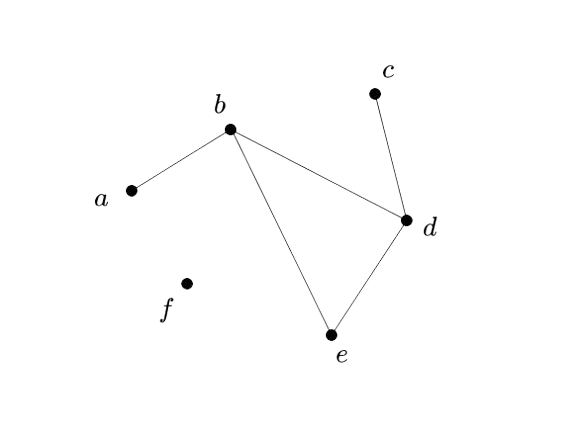
\includegraphics[width=\textwidth, height=5cm, keepaspectratio=true]{images/graph.jpeg}
    \captionof{figure}{Example of a (simple, undirected) graph with finite vertex and edge sets.}
    \label{fig:graph}
\end{center}

A \textbf{subgraph} of $G$ is a graph the vertex set and edge set of which are subsets of the vertex set and edge set of $G$ respectively.

\begin{center}
    \centering
    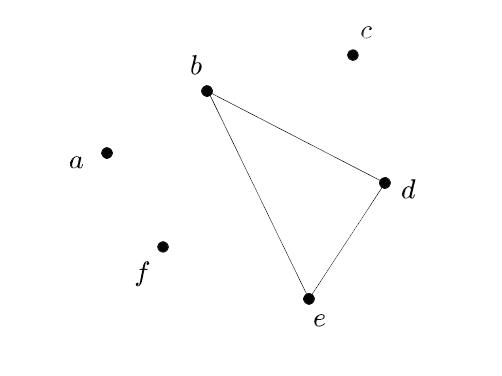
\includegraphics[width=\textwidth, height=5cm, keepaspectratio=true]{images/subgraph.jpeg}
    \captionof{figure}{Example of a subgraph of the graph shown in Figure \ref{fig:graph}.}
    \label{fig:subgraph}
\end{center}

If $xy$ is an edge, then $x$ and $y$ are said to be \textbf{adjacent} or that $y$ is a \textbf{neighbour} of $x$ and we denote it as $x \sim y$.

An \textbf{independent vertex set} of a graph $G$ is a subset of the vertices such that no two vertices in the subset are adjacent in $G$.

A vertex is \textbf{incident} with an edge if it is one of the two vertices of the edge. 

A simple graph is said to be \textbf{complete} if every pair of vertices are adjacent. The complete graph of $n$ vertices is usually denoted as $K_n$. $K_n$ has ${n \choose 2}$ edges.

\begin{center}
    \centering
    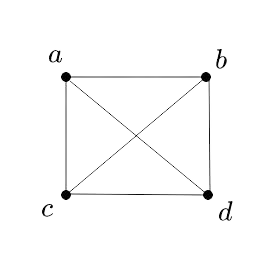
\includegraphics[width=\textwidth, height=4cm, keepaspectratio=true]{images/complete.jpeg}
    \captionof{figure}{Complete graph $K_4$.}
    \label{fig:complete}
\end{center}

The \textbf{degree} of a vertex $v \in V(G)$, denoted as $d(v)$ is the number of edges in $E(G)$ that are incident to $v$ taking into account that loops are considered twice, i.e. a vertex that is only adjacent to itself with a loop has degree $2$.

If $G$ is a graph, we denote by 
    \begin{enumerate}[label=\roman*.]
        \item $\delta(G) = \min \{d(v) : v \in V\}$ the \textbf{minimum degree} of $G$.
        \item $\Delta(G) = \max \{d(v) : v \in V\}$ the  \textbf{maximum degree} of $G$.
    \end{enumerate}

$G$ is a \textbf{regular graph of degree r} if $\delta = \Delta = r$. That is, all vertices have degree $r$. $K_4$ as shown in Figure \ref{fig:complete} is regular of degree 3.

\begin{lemma}(Euler's Handshake Lemma)
For every graph G, if we add the degrees of its vertices, we get twice the number of edges $m$. That is,
    \begin{equation*}
        \sum_{v \in V(G)} d(v) = 2m.
    \end{equation*}
\end{lemma}

\begin{proof}
We can prove this by induction on $m$. If $m=0$, the result is trivial. If $m=1$, then either $n=2$ and each of the two vertices has degree 1 or the edge is a loop and there is a single vertex of degree 2. In both cases, the equality we are trying to prove holds true. 

Now assume such equality is true for $m \leq k$ and let $G$ be a graph with $m=k+1$ edges. Consider any edge $e$ from $G$ and the graph $H = G - e$ (i.e. we remove edge $e$ from $G$). Then, every vertex in $H$ has the same degree as in $G$ except two vertices that have one degree less than they have in $G$ (if $e$ is not a loop) or there is only one vertex having two degrees less (if $e$ is a loop). 

In either case, using the induction hypothesis, we obtain: 
    \begin{equation*}
       \sum_{v \in V(G)} d(v) = \sum_{v \in V(H)} d(v) + 2 = 2(m-1) + 2 = 2m. 
    \end{equation*}
\end{proof}

\begin{lemma} \label{lemma2}
    If $G$ is a simple $n$-vertex graph, then $\sum_{u \in V} d(u) \leq n^2 - n$.
\end{lemma}

\begin{proof}
By the Handshake Lemma, the sum of the degrees of all vertices of a graph $G$ is equal to twice the number of edges of $G$. That is, $\sum_{u \in V} d(u) = 2m$, with $m = \# E(G)$. Moreover, a simple graph has, at most, ${n}\choose{2}$ edges. By putting all this together one obtains:

\begin{equation} 
\sum_{u \in V} d(u) = 2m \leq 2 {n \choose 2} = \frac{2(n-1)n}{2} = n^2 - n.
\end{equation}
\end{proof}

The \textbf{complement} of a graph $G$, denoted as $\overline{G}$, is the graph with the same vertex set as $G$ but with edge set consisting of the edges not present in $G$. That is, the edge set of $\overline{G}$ is the complement of the edge set of $G$. 

\begin{center}
    \centering
    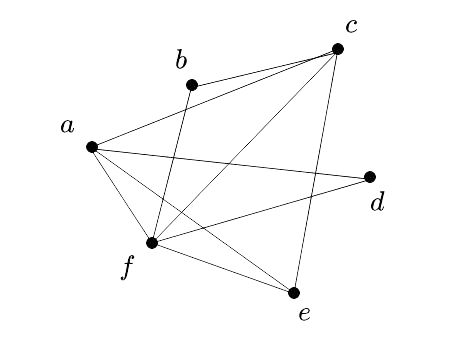
\includegraphics[width=\textwidth, height=4cm, keepaspectratio=true]{images/complement.jpeg}
    \captionof{figure}{Complement of the graph in Figure \ref{fig:graph}.}
    \label{fig:complement}
\end{center}

A \textbf{walk of length $k$} between the vertices $v_1,v_{k+1}$ of a given graph is a sequence of $k$ edges of the form $v_1 v_2, v_2 v_3, \ldots, v_k v_{k+1}$. In particular, this walk can also be denoted as $v_1 v_2 \ldots v_{k+1}$. If $v_1=v_{k+1}$, then it is a \textbf{closed walk of length $k$}.

A \textbf{cycle} is a closed walk of length $k$ where all edges and intermediate vertices are different. When a graph consists of only one cycle and no other vertices involved, it can be denoted as $C_k$, where $k$ is the number of vertices of such graph. For example, $C_3$ is a triangle and is known as the $\textbf{triangle graph}$. 

\begin{center}
    \centering
    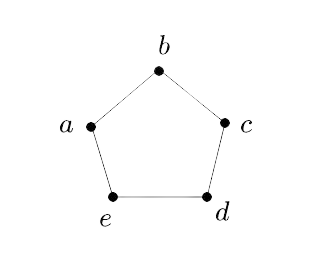
\includegraphics[width=\textwidth, height=4cm, keepaspectratio=true]{images/cycle.jpeg}
    \captionof{figure}{Cycle $C_5$.}
    \label{fig:cycle}
\end{center}

A \textbf{trail} is a walk for which all edges are different. A \textbf{path} is a trail for which all vertices are also different.

An \textbf{Eulerian tour} is a closed walk in $G$ that visits each edge exactly once. If $G$ has an Eulerian tour, $G$ is said to be an Eulerian graph.

A graph is said to be \textbf{connected} if there exists a path between every pair of vertices. $K_4$, shown in Figure \ref{fig:cycle}, is connected.

A connected graph with $n$ vertices is \textbf{unicyclic} if it has exactly $n$ edges. The triangle, $C_3$, is a unicyclic graph.  

Similarly, a connected graph with $n$ vertices and $n+1$ edges is \textbf{bicyclic}. 

\begin{center}
    \centering
    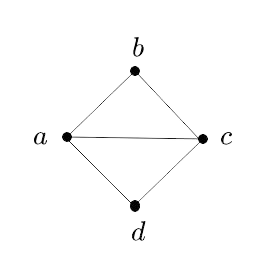
\includegraphics[width=\textwidth, height=4cm, keepaspectratio=true]{images/bicyclic.jpeg}
    \captionof{figure}{Example of a bicyclic graph.}
    \label{fig:bicyclic}
\end{center}

A \textbf{tree} is a connected graph with no cycles. 

\begin{center}
    \centering
    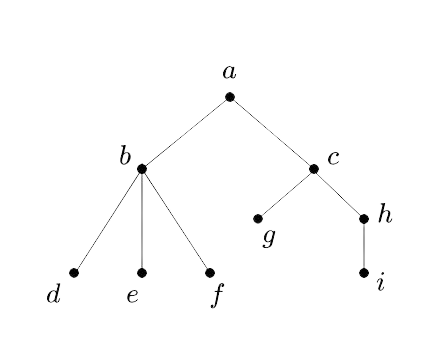
\includegraphics[width=\textwidth, height=5cm, keepaspectratio=true]{images/tree.jpeg}
    \captionof{figure}{Example of a tree graph.}
    \label{fig:cycle}
\end{center}

A \textbf{threshold graph} is a graph that can be constructed from a one-vertex graph by a sequence of operations of the form (i) add an isolated vertex or (ii) take the complement.

A \textbf{clique} of a graph $G$ is a complete subgraph of $G$.

A \textbf{split graph} is a graph the vertices of which can be partitioned into two disjoint sets $K$ and $I$ such that $K$ is a clique and $I$ an independent vertex set. Complete graphs are split graphs.

A \textbf{chord} of a graph cycle $G$ is an edge that connects two vertices of $G$ but that is not part of the edge set of $G$. The edge joining vertices $a$ and $c$ in Figure \ref{fig:bicyclic} is a chord of $C_4$

A \textbf{chordal graph} is a simple graph such that every graph cycle of length four and greater has a cycle chord.

If $G' \subseteq G$ and $G$ contains all edges $xy \in E(G)$ with $x, y \in V(G')$, then $G'$ is an \textbf{induced subgraph} of G. We say that $V(G')$ induces or spans $G'$ in $G$ and denote this as $G' =: G[V(G')]$. An \textbf{induced cycle} in $G$ is a cycle in $G$ forming an induced subgraph. Moreover, one can deduce that an induced cycle is one that has no chords. 

The following structural characterization of split graphs will be important in Section \ref{implementation} when looking for counterexamples to Conjecture \ref{brouwer}.

\begin{thm}
Let $G$ be a graph. Then $G$ is split if and only if $G$ and $\overline{G}$ are chordal. 
\end{thm}

\begin{proof} 
$\implies$ Suppose $G$ is split and contains a chordless cycle $C$ of length $\geq 4$. By definition of split graph, the vertices of $G$ can be partitioned into two disjoint sets $K$ and $I$ such that $K$ is a clique and $I$ an independent vertex set. At least $1$ vertex and at most $2$ vertices of $C$ are in $K$. Since any two vertices in $K$ are connected, as it is complete by definition, this implies that $I$ must contain at least $2$ connected vertices. Therefore, $G$ must be chordal. If $G$ is split, then $\overline{G}$ is also split, and so $\overline{G}$ must also be chordal. 

$\impliedby$ This proof is a consequence of Foldes and Hammer \cite{zbMATH03632548}. Suppose both $G$ and $\overline{G}$ are chordal. It follows that the largest induced cycles in both $G$ and $\overline{G}$ are triangles. Let $K$ be the maximum clique in $G$. If there are multiple maximum cliques, let $K$ be the clique such that $E(G[V(G)\setminus K])$, i.e. the edge set of the graph induced by $V(G)\setminus K$ is minimized. We show that no two vertices in $V(G)\setminus K$ are adjacent.

By contradiction. Suppose that $x$ and $y$ are two adjacent vertices in $V(G)\setminus K$. We can pick two distinct vertices $u, v \in K$ such that $x \not\sim u$ and $y \not\sim v$, i.e. $xu \not\in E(G)$ and $yv \not\in E(G)$. Clearly, neither $x$ nor $y$ are adjacent to all vertices in $K$, as this would imply that $K$ is not maximum. In addition, if $x$ and $y$ were adjacent to all vertices in $K$ except some vertex $z$, then we could form a larger clique $K' = K \setminus \{z\} \cup \{x, y\}$. 

We also claim that exactly one of the edges in $\{ xv, yu\}$ is in $E(G)$. If $xv, yu \in E(G)$, then $(x, y, u, v)$ would be an induced cycle $C_4$ in $G$. If neither edge was in $E(G)$, then $(x, y, u, v)$ would be an induced cycle $C_4$ in $\overline{G}$. Without loss of generality, we suppose that $yu \in E(G)$.

We claim that $y$ is adjacent to all vertices of $K$ except $v$. Otherwise, there would exist some vertex $w \in K$, $w \neq v$ such that $yw \not\in E(G)$. Either $x$ is adjacent to $w$ or $x$ is not adjacent to $w$. If $x \sim w$, then $(x, w, u, y)$ forms an induced cycle $C_4$ in $G$. If $x \not\sim w$, then $(x, v, y, w)$ is an induced cycle $C_4$ in $\overline{G}$.

So far, we have that $x, y \in V(G) \setminus K$, $xy \in E(G \setminus K)$, and $u, v \in K$. Further, without loss of generality we have that $y$ is adjacent to all vertices in $K$ except $v$, and $x$ is not adjacent to $u$ or $v$.

Now, we prove that all neighbors of $v$ in $V(G) \setminus K$ must be adjacent to $y$. Suppose otherwise and let $t$ be a vertex in $V(G) \setminus K$ adjacent to $v$ and not adjacent to $y$. If $t \not\sim x$ then $(x, t, y, v)$ would form an induced cycle $C_4$ in $\overline{G}$. However, if $t \sim x$, then $(x, t, v, u, y)$ forms an induced cycle $C_5$ in $G$.

With what we have shown so far, we can construct another clique $K'$ in $G$ that provides a smaller edge set in the graph induced by $V(G) \setminus K'$, yielding a contradiction to the minimality in the choice of $K$.

Let this graph be $K' = K \setminus \{v\} \cup y$, then the edge set of the graph induced by $V(G) \setminus K'$ contains at least one fewer edge than the graph induced by $V(G) \setminus K$. That is, the edge $xy$ is lost and we do not gain a corresponding edge $xv$. This is a contradiction and therefore no two vertices in $V(G) \setminus K$ are adjacent. 
\end{proof}

A \textbf{directed graph} is a graph in which the edges have a direction. Such direction is usually indicated with an arrow on the edge.

\begin{center}
    \centering
    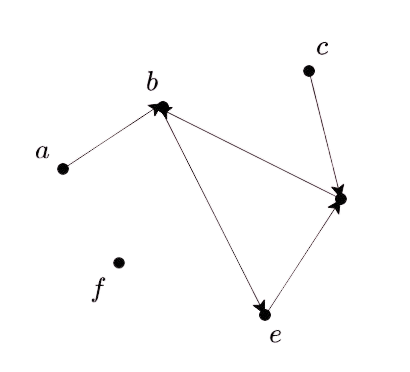
\includegraphics[width=\textwidth, height=5cm, keepaspectratio=true]{images/directed.jpeg}
    \captionof{figure}{Example of a directed graph.}
    \label{fig:directed}
\end{center}

Graphs that are not directed are called \textbf{undirected graphs}. All graphs discussed in this thesis are assumed to be undirected. 

\textbf{Vertex coloring} is the process of assigning colors to the vertices of a graph such that no two adjacent vertices get the same color label. Similarly, \textbf{edge coloring} is an assignment of colors to the edges of a graph such that no two incident edges have the same color.

\begin{figure}[H]
   \begin{minipage}{0.45\textwidth}
     \centering
     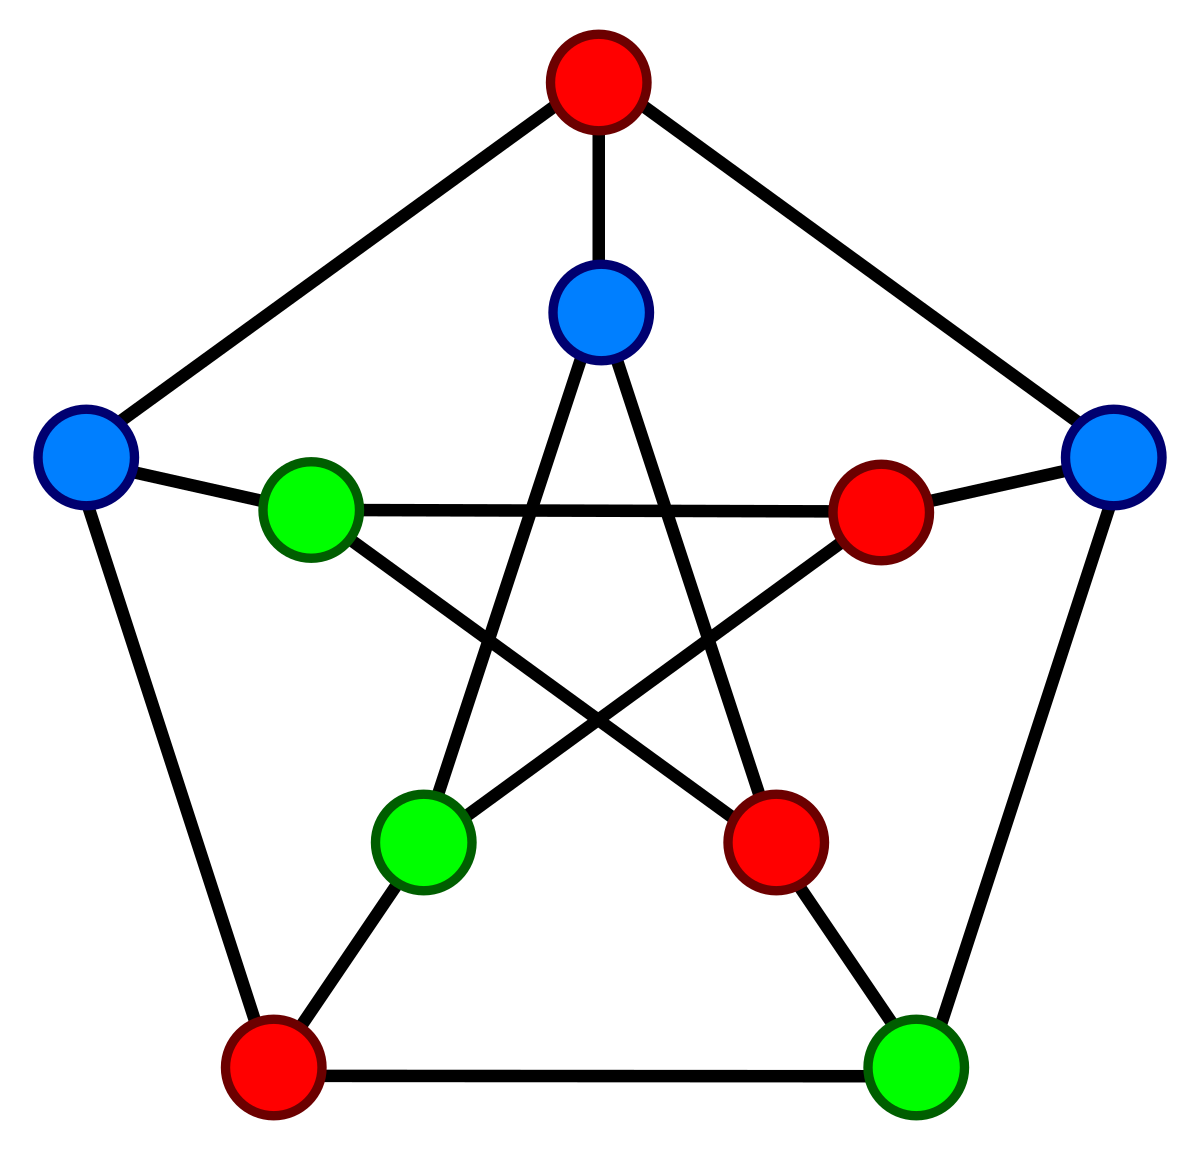
\includegraphics[width=.5\linewidth]{images/vertex_coloring.jpeg}
     \caption{Example of a vertex coloring of the Petersen graph.}\label{fig:vertex_coloring}
   \end{minipage}\hfill
   \begin{minipage}{0.5\textwidth}
     \centering
     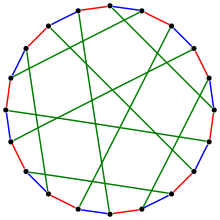
\includegraphics[width=.45\linewidth]{images/edge_coloring.jpeg}
     \caption{Example of an edge coloring of the Desargues graph.}\label{fig:vertex_coloring}
   \end{minipage}
\end{figure}

\begin{defn} \label{snark}
A \textbf{snark} is an undirected graph with exactly three edges per vertex whose edges cannot be colored with only three colors. 
\end{defn}

A subset $M \subset E(G)$ is a \textbf{matching} of $G$ if any pair of edges in $M$ are not adjacent. That is, a matching is a set of edges without common edges. A \textbf{matching} $M$ covers a vertex $v \in V(G)$ if there exists an edge in $M$ incident at $v$.

$M$ is a \textbf{perfect matching} if it covers all vertices of $G$. $M$ is a \textbf{maximum matching} if there does not exist another matching $M'$ with a larger number of edges. If $M$ is a perfect matching, then it is also a maximum matching. However, the converse is not generally true.

\begin{figure}[H]
   \begin{minipage}{0.5\textwidth}
     \centering
     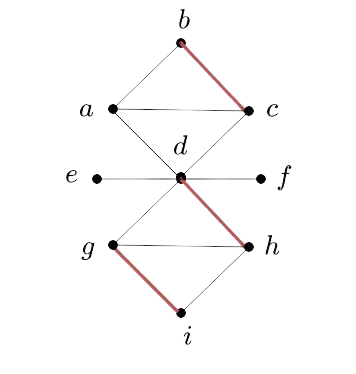
\includegraphics[width=.65\linewidth]{images/maximum_matching.jpeg}
     \caption{Example of a maximum matching.}\label{fig:maximum_matching}
   \end{minipage}\hfill
   \begin{minipage}{0.5\textwidth}
     \centering
     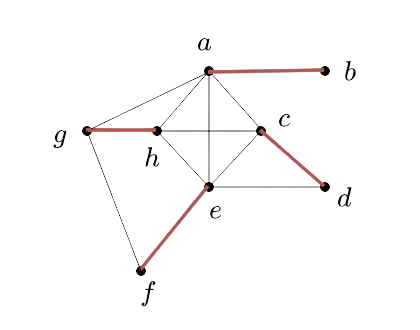
\includegraphics[width=.8\linewidth]{images/perfect_matching.jpeg}
     \caption{Example of a perfect matching.}\label{fig:perfect_matching}
   \end{minipage}
\end{figure}

The number of edges in a maximum matching is referred to as \textbf{matching number} and is usually denoted as $\mu$.

\subsection{Spectral Graph Theory}

All graphs have several matrix representations associated and, by studying such matrices and their invariants, one may learn important characteristics about those graphs. Here are some key notions and results in the field of linear algebra and spectral graph theory.

Let us recall that a matrix $A$ is \textbf{symmetric} if it satisfies $A^T = A$, where $A^T$ refers to the transpose matrix of $A$, and that the \textbf{spectrum} of a matrix is the set of its eigenvalues. Moreover, the \textbf{spectral radius} of a square matrix is the maximum of the absolute values of its eigenvalues.

Here we present some necessary properties of symmetric matrices.

\begin{lemma}
Let $A$ be a real symmetric matrix. If $u$ and $v$ are eigenvectors of $A$ with different eigenvalues, then $u$ and $v$ are orthogonal.
\end{lemma}

\begin{proof}
Suppose that $A u = \lambda u$ and $A v = \tau v$. As $A$ is symmetric, $u^T A v = (v^T A u)^T$. However, the left-hand side of this equation is $\tau u^T v$ and the right-hand side is $\lambda u^T v$, and so if $\tau \neq \lambda$, it must be the case that $u^T v = 0$.
\end{proof}

\begin{lemma}
The eigenvalues of a symmetric matrix $A$ are real numbers.
\end{lemma}

\begin{proof}
Let $u$ be an eigenvector of $A$ with eigenvalue $\lambda$. Then, by taking the complex conjugate of the equation $Au = \lambda u$ we get $A \overline{u} = \overline{\lambda} \overline{u}$ and so $\overline{u}$ is also an eigenvector of $A$. By definition, $u, \overline{u} \neq 0$ so $u^{T} \overline{u} > 0$. By the previous lemma, $u$ and $\overline{u}$ cannot have different values so $\lambda = \overline{\lambda}$ and the claim is proved. 
\end{proof}

Due to its length and the need to prove some intermediate results, the proof of the below theorem is beyond the scope of this thesis. One can find its proof in Chapter 8 of \cite{Bretscher}, Theorem 8.1.3.

\begin{thm} \label{spectral theorem consequence}
A symmetric $n \times n$ matrix $A$ has $n$ real eigenvalues, accounting for their algebraic multiplicities.
\end{thm}

Let $G$ be a graph. The \textbf{adjacency matrix} $A$ of a graph $G$ is the 0-1 matrix with rows and columns indexed by the vertices of $G$ such that $A_{xy} = 1$ if $x$ and $y$ are adjacent and $A_{xy} = 0$ otherwise. The adjacency matrix is a $n \times n$ square matrix (i.e. it has $n$ rows and $n$ columns), with $n$ being the number of vertices of the graph. Moreover, the adjacency matrix is also symmetric.  

Let $G$ be an undirected graph. The \textbf{incidence matrix} $B$ of a graph $G$ is the 0-1 matrix with rows indexed by the vertices and columns indexed by the edges, where $B_{xe} = 1$ if vertex $x$ is incident to edge $e$ and $B_{xe} = 0$ otherwise. For directed graphs, we have that the directed incidence matrix which not only consists of 0' and 1's as elements but also -1's. Depending on the direction of a given edge, its corresponding entry in the directed incidence matrix will be 1 or -1.  

The \textbf{degree matrix} $D$ of a graph $G$ is the square matrix that represents the degree of all vertices of such graph. If $v_1, ..., v_n$ are the vertices of $G$, the degree matrix takes the following form:

\begin{equation*}
    \begin{bmatrix}
        d(v_1) & \cdots & 0 \\
        \vdots & \ddots & \vdots \\
        0 & \cdots & d(v_n) 
    \end{bmatrix}.
\end{equation*}

\bigskip

\begin{defn}
The \textbf{Laplacian matrix} of a graph $G$, denoted as $L$, is the square matrix $D - A$, where $D$ and $A$ are the degree and the adjacency matrix of $G$, respectively. The matrix $Q = D + A$, also square, is called \textbf{signless Laplacian} of $G$.
\end{defn}

We present the following lemma as it is useful for another result. However, its proof is beyond the scope of this thesis.

\begin{lemma}
Both the Laplacian and signless Laplacian matrices of a graph $G$ are positive semidefinite as we can express them as $L = NN^T$ and $Q = BB^T$, where $B$ is the incidence matrix of $G$ and $N$ the directed incidence matrix of the directed graph obtained by orienting the edges of $G$ in an arbitrary way.
\end{lemma}

Usually, the (ordinary) spectrum of a finite graph $G$ is by definition the spectrum of the adjacency matrix $A$ and the \textbf{Laplace spectrum} of a finite undirected graph is the spectrum of the Laplace matrix $L$.  

Note that for an undirected graph, the adjacency matrix and the Laplacian matrix are symmetric. Therefore, by Theorem \ref{spectral theorem consequence}, $L$ has $n$ real eigenvalues, being $n$ the number of vertices of $G$. 

The \textbf{distance} between two vertices $x$ and $y$ of a graph $G$, denoted as $d_{xy}$, refers to the length of a shortest path between $x$ and $y$ in $G$ and it is $+\infty$ if there is no path.  
\begin{defn}
The \textbf{distance matrix} $D'$ of a graph $G$ is the matrix with rows and columns indexed by the vertices of G such that the $xy$-entry corresponds to the distance between the vertices $x$ and $y$. 
\end{defn}

Let us note that for a connected graph $G$ the function $d:V\times V\to \mathbb{N}$ is a metric, in particular
all distance matrices have $0$'s in the diagonal. Moreover, they are symmetric.

Let $G$ be a graph with vertex set $V(G)$. The \textbf{transmission} $Tr(x)$ of a vertex $x$ is defined as the sum of the distances from $x$ to all other vertices of that graph. That is, $Tr(x) = \sum_{y \in V(G)} d_{xy}$. 

\begin{defn}
The \textbf{distance Laplacian} of a connected graph $G$ is the matrix $D^L = T - D'$, where T is the diagonal matrix with $Tr(x_i)$ in the $i$-th diagonal entry.
\end{defn}

The proof of the following theorem can be found in \cite{shi}.

\begin{thm} \label{spectral radius}
Let G be a graph with vertex set $V(G)$ and edge set $E(G)$, $\lambda$ the spectral radius and $d(u)$ the degree of vertex $u \in V(G)$. Then, 
\begin{equation*}
    \lambda \leq \max_{v \in V}{\big(\sum_{uv \in E} d(u)\big)^{1/2}}.
\end{equation*}
\end{thm}

\begin{obs}
Given Theorem \ref{spectral radius} and Lemma \ref{lemma2}, one can easily see that
\begin{equation} \label{eq2}
    \lambda \leq \max_{v \in V}{\big(\sum_{uv \in E} d(u)\big)^{1/2}} <  \big(\sum_{u \in V} d(u) \big)^{1/2} \leq (n^2 - n)^{1/2} < n.
\end{equation}
\end{obs}

\newpage

% Graph Theory Conjectures
\section{Graph Theory Conjectures} \label{conjectures}

In mathematics, a \textbf{conjecture} is a formal statement or proposition that is believed to be true but that has not been proved yet. When a conjecture is proved to be true, it becomes a \textbf{theorem}. 

Conversely, to disprove a conjecture, it suffices to find a counterexample or to show that such conjecture contradicts a statement previously proven to be true. One then says that the conjecture is \textbf{false}.

Researchers in mathematics work on trying to prove or disprove conjectures, some of them being very old statements that have been unsolved for decades. This section explores some ways to \textit{create} new conjectures using a computer and gives some such conjectures from spectral graph theory.

\subsection{Finding Graph Theory Conjectures Using Mathematical Software}

Often times conjectures appear after mathematicians notice a pattern that holds true for many cases, thus indicating that such pattern may always hold. In some fields within mathematics, graph theory being one of them, mathematicians use software packages to discover new conjectures. This shows that computers can help mathematics move forward by not only assisting mathematicians in proving or disproving results but by giving mathematicians hints about possibly true statements.

The first system for automated discovery of conjectures used by graph theorists is \textbf{GRAPH}, an interactive programming system for the classification and extension of knowledge in the field of graph theory. This system was developed and built at the Faculty of Electrical Engineering at the University of Belgrade in the early 1980s by Dragoš Cvetković and other collaborators \cite{zbMATH05689445}. GRAPH allowed mathematicians to find conjectures and prove theorems in graph theory, especially in spectral graph theory. 

In recent years, graph theorists have been obtaining new conjectures from more modern systems for automated conjecture discovery. Two examples of such newer systems are \textbf{Graffiti} and \textbf{AutoGraphiX}, referenced by Wagner in \cite{Wagner:2021} and Roucairol and Cazenave in \cite{RoucairolCazenave:2022}. 

In broad terms, most automated conjecture discovery systems are based on one of the following principles: 

\begin{itemize}[label=\raisebox{0.25ex}{\tiny$\bullet$}]
    \item The system takes advantage of the ability of the computer to perform fast computations involving the values of invariants of a series of graphs or expressions containing such invariants, i.e. the GRAPH system.
    \item The system exploits compilations of relationships between graph invariants. For several classes of graphs it substitutes constant or equivalent expressions for graph invariants, as in constraint programming tasks or routines.
    \item The system generates several conjectures of a simple form (i.e. inequalities between two invariants or between an invariant and the sum of two other invariants) and then selects those which are interesting. That is, the ones that cannot be implied by previously known conjectures, do not contradict any results known to be true and those the system itself is not able to falsify. Graffiti is one of such systems. All conjectures created by Graffiti appear in the website Written in the Wall \cite{WrittenWall}, which documents the status of nearly 1000 conjectures.
    \item The system enumerates all graphs of given classes, possibly exploiting symmetry. If a property cannot be disproved by small counterexamples, then the system creates a conjecture from such property. 
    \item The system uses heuristic optimization tools to identify extremal or near-extremal families of graphs classes of graphs which are extremal or near extremal for some invariants or expressions that act as constraints. It then studies such families and deduces conjectures from them, i.e. the AutoGraphiX system.
\end{itemize}

Many conjectures obtained from automated conjecture discovery systems and their proofs or refutations have ended up becoming pieces of work published in several journals, showing that these systems really do make mathematics advance.
More about automated conjecture discovery can be found in \cite{zbMATH05689445} and \cite{zbMATH02041897}. 

\subsection{Some Spectral Graph Theory Conjectures} \label{subsection conjectures}

In this subsection we introduce the spectral graph theory conjectures we try to disprove.

In the following section we will see how these conjectures can be translated to problems a reinforcement learning can understand and dive into the end-to-end implementation of such problems. 

\begin{conj}\label{wagner}
    Let $G$ be a connected graph with $n \geq 3$ vertices, with largest eigenvalue $\lambda^*$ and matching number $\mu$. Then 
    \begin{equation*}
        \lambda^* + \mu \geq \sqrt{n-1} + 1.
    \end{equation*}
\end{conj}

\begin{obs}
    When we talk about the eigenvalues of a graph (i.e. without specifying its matrix representation), we will assume that these eigenvalues are the eigenvalues of that graph's adjacency matrix. 
\end{obs}

Conjecture \ref{wagner} first appeared in \cite{zbMATH05689445} and was originally obtained from AutoGraphiX. This same conjecture was refuted by Stevanović in \cite{zbMATH05804421}, where he noted that there exists an infinite family of counterexamples. However, he did not use a learning-powered approach as Wagner did and the counterexample given by Stevanović was a larger graph ($n = 600$ vertices) than the one Wagner found ($n = 19$ vertices). Moreover, Wagner notes that this conjecture appears to be true for graphs with $n \leq 18$ vertices.

The second conjecture we will be working with is \textbf{Brouwer's conjecture}. Prior to presenting it in this thesis, we need to introduce some results.

%\begin{prop}
    %Let $G$ be a threshold graph with Laplace eigenvalues (i.e. the eigenvalues of the Laplacian matrix) in non-increasing order $\lambda_1 \geq \lambda_2 \geq \cdots \geq \lambda_n = 0$. Let $d(v)$ be the degree of vertex $v$. Then,
    %\begin{center}
        %$\lambda_j = \#\{ v \mid d(v) \geq j\}$.
    %\end{center}
%\end{prop}

%\begin{proof}
%This proposition can be proved by induction on the number of construction steps of type (i) and (ii). 
%\end{proof}

The following was conjectured by Grone and Merris in \cite{GroneMerris} and proved to be true by Hua Bai in \cite{HuaBai}.

\begin{thm}(Grone-Merris)
    For all undirected graphs and all $t = \{1, ..., n\}$ the following inequality holds 
    \begin{equation*}
        \sum_{j=1}^{t} \lambda_j \leq \sum_{j=1}^{t} \#\{ v \mid d(v) \geq j\}.
    \end{equation*}
\end{thm}

For $t=1$ this is immediate by Expression (\ref{eq2}). Moreover, for $t = n$ the equality holds.

In \cite{BrouwerHaemers:2011}, the authors present the following conjecture, which is a variation of the Grone-Merris theorem.

\begin{conj}[Brouwer]\label{brouwer}
Let $G$ be a graph with $n$ vertices, $e$ edges and Laplace eigenvalues $\lambda_1 \geq \lambda_2 \geq \cdots \geq \lambda_n = 0$. Then, for each $1 \leq t \leq n$ it is true that 
\begin{equation*}
    \sum_{i=1}^{t} \lambda_i \leq e + {t+1 \choose 2}.
\end{equation*}
\end{conj}

The above result is stronger than the Grone-Merris theorem for some $t$ if and only if the graph is not a split graph \cite{Mayank}.

Conjecture \ref{brouwer} is known to be true for threshold graphs, despite the fact that such proof is not included in \cite{GroneMerris}. Nonetheless, the authors state that it can be proved by induction. 

Moreover, this conjecture is known to be true for: 
\begin{itemize}[label=\raisebox{0.25ex}{\tiny$\bullet$}]
    \item $t=1$, see Expression (\ref{eq2});
    \item $t=2$ \cite{Haemers:Mohammadian};
    \item $t=n$ and $t=n-1$ \cite{Wang:Huang:Liu};
    \item trees \cite{Fritscher:Hoppen:Rocha:Trevisan};
    \item unicyclic and bicyclic graphs \cite{DuZhou:2012,Wang:Huang:Liu};
    \item regular graphs \cite{Berndsen,Mayank};
    \item split graphs \cite{Berndsen,Mayank};
    \item cographs \cite{Berndsen,Mayank};
    \item graphs with $n \leq 10$ vertices \cite{Berndsen,Mayank}.
\end{itemize}

In \cite{Chen:2019} Chen also shows that when Brouwer's conjecture holds for $t=p$ with $1 \leq p \leq (n-1)/2$, then it is also true for $t=n-p-1$. Further, Cooper finds in \cite{Cooper:2020} several constraints for several types of graphs regarding Brouwer's conjecture.

There exist several variants to Brouwer's conjecture:

\begin{conj}\label{signless}
Let $G$ be a graph with $n$ vertices and $e$ edges such that the \textbf{signless} Laplacian has eigenvalues $\lambda_1 \geq \lambda_2 \geq \cdots \geq \lambda_n = 0$. Then, for each $1 \leq t \leq n$ it is true that 
\begin{equation*}
    \sum_{i=1}^{t} \lambda_i \leq e + {t+1 \choose 2}.
\end{equation*}
\end{conj}

This variant to Brouwer's conjecture is proposed by Ashraf, Omidi, and Tayfeh-Rezaie in \cite{Ashraf:Omidi:Tayfeh-Rezaie}. In this same paper, the authors prove this conjecture is true for $t=1,2,n-1,n$ for all graphs and for all $t$ for regular graphs and for trees. Moreover, they also check by computation that it holds for all graphs up to 10 vertices.

Finally, we present one final variant to Brouwer's conjecture. Nonetheless, trying to find a counterexample for it is beyond the scope of this thesis.

\begin{conj}\label{signless distance}
Let $G$ be a graph with $n$ vertices and $e$ edges such that the \textbf{signless distance} Laplacian has eigenvalues $\lambda_1 \geq \lambda_2 \geq \cdots \geq \lambda_n = 0$. Then, for each $1 \leq t \leq n$ it is true that 
\begin{equation*}
    \sum_{i=1}^{t} \lambda_i \leq e + {t+1 \choose 2}(n-\frac{2t+1}{3}).
\end{equation*}
\end{conj}

This conjecture is proposed by Alhevaz, Baghipur, Ganie and Pirzada in \cite{Alhevaz:Baghipur:Ganie:Pirzada}.

It would be natural to study a variant of Conjecture \ref{signless distance} for the distance Laplacian as well but no conjecture has been published about this.

\newpage

% Machine Learning Preliminaries 
\section{Machine Learning Preliminaries} \label{machine learning}

This section assumes the reader is familiar with basic concepts of probability and statistics, such as random variables and conditional probabilities.

\subsection{Introduction to Machine Learning}

\textbf{Artificial Intelligence}, usually abbreviated as AI, is defined as the capability of a machine to behave as if it had human intelligence. AI systems are capable of performing complex tasks in a way that is similar to how problems are solved by humans.

\textbf{Machine learning} is a subfield of AI that provides a system with the ability to gain or acquire knowledge and improve from experience without being explicitly programmed to do so, in contrast to traditional computational approaches to a problem. The term machine learning was first coined in the 1950s by Arthur Samuel \cite{Samuel}, a computer scientist who developed a computer program to play checkers and realized that the more the machine played, the better it performed. 

Despite the fact that it is a continuously developing discipline, machine learning is already being used to solve many real-world problems in a vast variety of fields, including healthcare, logistics and banking. Moreover, machine learning has advanced dramatically in the last two decades, going from something that only existed in research centers to a technology that has widespread commercial uses. Recent progress in this discipline has been motivated both by the development of new learning algorithms and the larger availability of data and lower storage and computation costs.

Machine learning lies at the intersection of statistics and computer science. We now present some key definitions that are useful to understand machine learning concepts.

Let us recall that given an arbitrary set $\mathcal{X}$, a collection $\mathcal{A}$ of subsets of $\mathcal{X}$ is a \textbf{$\sigma$-algebra} on $\mathcal{X}$ if: 
\begin{enumerate}[label=\roman*.]
    \item $\mathcal{X} \in \mathcal{A}$,
    \item for each set $A \in \mathcal{A}$, then $A^c \in \mathcal{A}$, where $A^c$ is the complement of set A,
    \item for each infinite sequence $\{A_i\}$ of sets that belong to $\mathcal{A}$, the set $\bigcup^{\infty}_{i=1}A_i$ belongs to $\mathcal{A}$, and
    \item for each infinite sequence $\{A_i\}$ of sets that belong to $\mathcal{A}$, the set $\bigcap^{\infty}_{i=1}A_i$ belongs to $\mathcal{A}$.
\end{enumerate}

A \textbf{measurable space} is a pair $(\mathcal{X}, \mathcal{A})$ where $\mathcal{X}$ is a set and $\mathcal{A}$ a $\sigma$-algebra of subsets of $\mathcal{X}$. Let $(\mathcal{X}, \Sigma)$ and $(\mathcal{Y}, T)$ be measurable spaces. A function $f: \mathcal{X} \rightarrow \mathcal{Y}$ is said to be \textbf{measurable} if for every $E \in T$, then $f^{-1}(E) := \{x \in \mathcal{X} | f(x) \in E\} \in \Sigma$. For measurable spaces $\mathcal{X}$ and $\mathcal{Y}$ we define $\mathcal{M}(\mathcal{X}, \mathcal{Y})$ to be the set of measurable functions from $\mathcal{X}$ to $\mathcal{Y}$.

Further, a (finite) collection of random variables $\{X_1, ..., X_n\}$ is \textbf{mutually independent} if and only if for any sequence of numbers $\{x_1, ..., x_n\}$, the events $\{X_1 \leq x_1\}, ..., \{X_n \leq x_n\}$ are mutually independent events. That is, for every $k \leq n$ and for every $k$ indices $1 \leq i_1 \leq ... \leq i_n$,
\begin{equation*}
    P\Big( \bigcap_{j=1}^k A_{i_j} \Big) = \prod_{j=1}^k P(A_{i_j}),
\end{equation*}
where $P(A)$ is the probability of event $A$ taking place.

A (finite) collection of $n$ random variables $\{X_1, ..., X_n\}$ is said to be \textbf{independent and identically distributed}, denoted as i.i.d, if each variable has the same probability distribution as the other variables and is mutually independent.

Formally, \textbf{learning} can be defined in the following way.

\begin{defn}
Let $\mathcal{X}, \mathcal{Y}$ and $\mathcal{Z}$ be measurable spaces. In a learning task, one is given data in $\mathcal{Z}$ and a loss function $\mathcal{L}: \mathcal{M}(\mathcal{X}, \mathcal{Y}) \times \mathcal{Z} \rightarrow \mathbb{R}$. The goal is to choose a hypothesis set $\mathcal{F} \subset \mathcal{M}(\mathcal{X}, \mathcal{Y})$ and construct a learning algorithm which is a mapping
\begin{equation*}
    \mathcal{A}: \bigcup_{m \in \mathbb{N}} \mathcal{Z}^m \rightarrow \mathcal{F},
\end{equation*}
that uses training data $s = (z^{(i)})_{i=1}^m \in \mathcal{Z}^m$ to find a model $f_s = \mathcal{A}(s) \in \mathcal{F}$ that performs well on the training data $s$ and also generalizes to unseen data $z \in \mathcal{Z}$. Performance is measured using the loss function $\mathcal{L}$ and generalization means that the out-of.sample performance of $f_s$ at $z$ behaves similar to the in-sample performance on $s$. Further, we are assuming that $z^{(1)}, ...,  z^{(m)}, z$ are realizations of i.i.d random variables $Z^{(1)}, ..., Z^{(m)}, Z$.
\end{defn}

Most machine learning problems belong to one of the three following paradigms, depending on the availability of an output variable in the data as well as on how the machine learning model is trained. 

\begin{itemize}[label=\raisebox{0.25ex}{\tiny$\bullet$}]
    \item In methods belonging to the \textbf{supervised learning} paradigm there is an outcome, also referred to as response or target variable, in the data that is being measured. The goal is to predict that outcome or to determine to which class or category it belongs. The data in supervised learning problems is said to be \textbf{labelled}. Given a set of data, one must split it into two sets. Part of this data (usually about $80\%$ of the original dataset) is used to train the model, while the remaining data is used to test how well the model can predict the desired outcome or how well it generalizes and classifies observations. A linear regression for prediction purposes is an example of a supervised learning method.
    
    \item The \textbf{unsupervised learning} approach does not deal with labelled data but instead aims at recognizing patterns that exist within the data in order to infer rules from them. In a sense, there is nothing being predicted. Typical unsupervised learning problems are clustering, association and dimensionality reduction.
    
    \item A third paradigm is \textbf{reinforcement learning}, which lies in the middle of supervised and unsupervised learning as the algorithm is only provided with a response showing how well the system is performing. The system learns from continuous feedback and it does not receive a dataset as in the other two paradigms. Instead, the data the system uses is generated as more iterations of the algorithm take place. Reinforcement learning is studied in more detail in section \ref{reinforcement}.
\end{itemize}

Machine learning problems can be classified into several categories, depending on what they are trying to solve. The main types of machine learning problems are the following.

\begin{itemize}[label=\raisebox{0.25ex}{\tiny$\bullet$}]
    \item \textbf{Classification} problems belong to the supervised learning paradigm. The response variable of such problems is a categorical variable that consists of two or multiple categories or classes. We classify a given observation into one of these categories.

    \item Another type of problems that belong to the supervised learning paradigm are \textbf{regression} problems. As opposed to classification problems, regression problems deal with numerical or continuous target variables to predict.

    \item \textbf{Clustering} problems fall under the unsupervised learning paradigm. In this type of problems, models try to learn the underlying structure of the data and compute how similar a set of observations are.

    \item \textbf{Reinforcement learning} problems, which are studied in more detail in section \ref{reinforcement}. 
\end{itemize}

\subsection{Introduction to Deep Learning}

This subsection presents basic concepts and notions to get started in deep learning, an extremely popular machine learning subfield. More about the field of deep learning can be read in \cite{buduma, nielsen, goodfellow}. A good resource to read about the mathematics behind deep learning is \cite{modern_math}.

One cannot talk about deep learning without first discussing neural networks. The \textbf{neuron} is the foundational unit of the human brain. Each neuron receives information from other neurons, processes this information in a unique way and sends the result to other neurons. We can translate this into an artificial model that can be represented on a computer. Just as biological neurons do, artificial neurons can take a given set of inputs $x_1, x_2, ...,  x_n$ multiplied by a specific weight $w_1, w_2, ..., w_n$. These weighted inputs are summed together and passed to a function $f$ to produce an output $y = f(z)$, where $z = \sum_{i=0}^n w_ix_i + b$ and $b$ is referred to as the \textbf{bias}. The output of a neuron is either 0 or 1, determined by whether $z$ is above or below an arbitrarily set threshold $\alpha$. That is,   

\begin{equation*}
    y = \begin{cases} 0, & \text{if }  z \leq \alpha \\ 1, & \text{otherwise} \end{cases}.
\end{equation*}

This can be thought of a binary classification problem since there exist two classes, 0 and 1, and we need to classify $y$ into one of them. Moreover, the threshold can be understood as the minimum probability of $y$ belonging to class 1 for $y$ to be considered to actually belong to class 1.  

This simple neuron structure can be represented in the following diagram:

\begin{center}
    \centering
    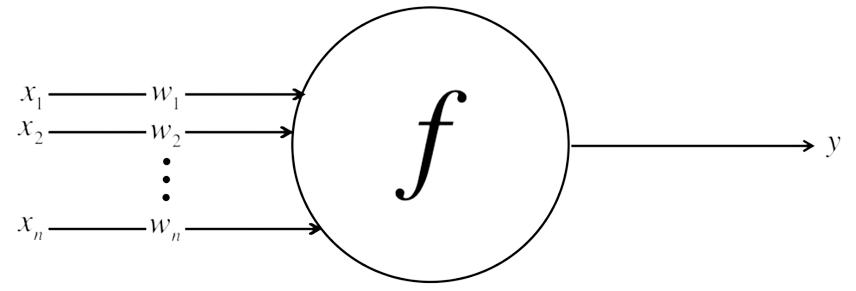
\includegraphics[width=\textwidth, height=3.5cm, keepaspectratio=true]{images/neuron.png}
    \captionof{figure}{Example of an artificial neuron, from \cite{buduma}.}
    \label{fig:neuron}
\end{center}

Sometimes, $f$ is denoted as $\sum$.

Artificial neurons as the one presented above were developed in the 1950s and 1960s by F. Rosenblatt \cite{rosenblatt}, who was inspired by previous work done by W. McCulloch and W. Pitts \cite{McCulloch:Pitts}. Nowadays, however, it is more common to use more sophisticated artificial neuron models.

So far, one could say that this characterization of artificial neurons bears an important resemblance to a linear regression specification and this is partly true because a single neuron only allows us to solve linear problems. 

To solve more complex (i.e. non-linear) problems one can can have several neurons organized in a sequential manner. Just as neurons in the human brain are organized in multiple layers and information flows (input) from one layer to another until sensory input is converted into conceptual understanding (final output), one can construct an artificial neural network consisting of several layers of neurons passing information to one another sequentially. Such architecture is known as \textbf{(artificial) neural network}. The first layer of neurons of a neural network is referred to as \textbf{input layer}, while the last layer is the \textbf{output layer}. Sometimes, there exist intermediate layers and these are called \textbf{hidden layers}. A \textbf{dense layer} is a type of hidden layer where every neuron is connected to all neurons in the next layer. \textbf{Deep neural networks} are neural networks that have several hidden layers. \textbf{Deep learning} is a subfield of machine learning dealing with deep neural network constructions.

The following diagram shows a neural network with five layers (where three of them are hidden) consisting of several neurons. 

\begin{center}
    \centering
    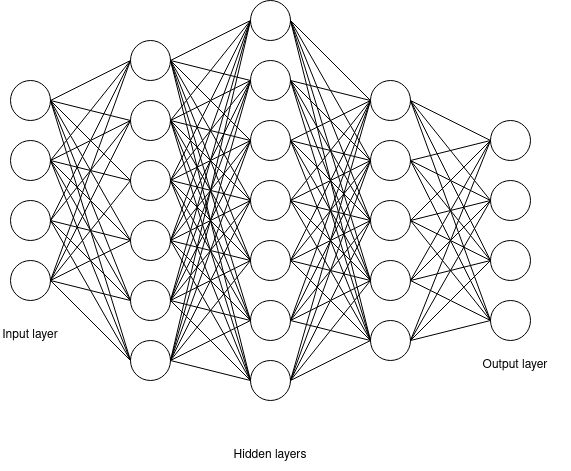
\includegraphics[width=\textwidth, height=7cm, keepaspectratio=true]{images/neural_network.png}
    \captionof{figure}{Example of a neural network with hidden layers.}
    \label{fig:neural_network}
\end{center}

We observe that neurons belonging to the same layer are not connected and there are no connections transmitting data from a higher layer (more to the right) to a lower layer (more to the left). Neural networks that satisfy this are called \textbf{feed-forward} networks.

However, if the problem we are solving is not linear and we build a neural network using only what we have presented so far, we will not necessarily outperform a single neuron since the sum of several linear specifications yields a linear result as well. Thus, in some settings, building a larger network does not guarantee getting more accurate results.

To solve this problem, one can modify the neural network structure to introduce some non-linearity. This is done with the so-called \textbf{activation functions}. These functions distort the output of a neuron to add non-linearities. A neuron with an activation function looks like in the following diagram:

\begin{center}
    \centering
    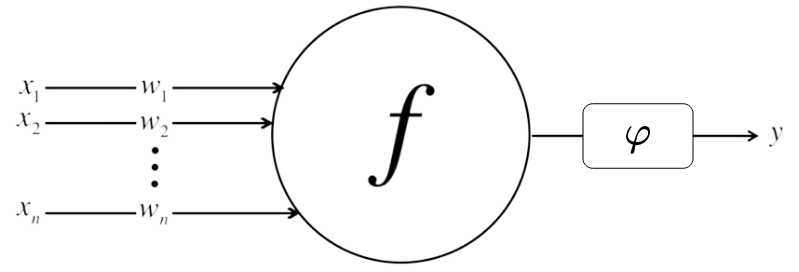
\includegraphics[width=\textwidth, height=3.5cm, keepaspectratio=true]{images/activation_function.png}
    \captionof{figure}{Example of the same neuron from Figure \ref{fig:neuron} with an activation function.}
    \label{fig:activation_function}
\end{center}

Non-linear activation functions $\varphi$ are applied to the output of a neuron to modify such output and constrain the values it takes into a given range. All neurons of a given layer have the same activation function and different layers can have different activation functions. When we add a non-linear activation function to a neural network, we are not summing only linear specifications so now we are able to build a neural network model that better approximates a non-linear output. The table in Appendix \ref{apx:activation} shows the most used activation functions.

%Let us note that a single neuron that solves a linear classification problem such as the one shown in Figure \ref{fig:neuron} is known as \textbf{perceptron}. Similarly, a neural network such as in Figure \ref{fig:neural_network} without any activation functions is referred to as \textbf{multilayer perceptron} and it is also used as a model for binary classification. Moreover, multilayer perceptrons are always feed-forward. Perceptrons are not used as much nowadays in favor of more complex and more accurate models. \kolja{o sea es perceptron cuando no hay activation function?}

Formally, the information presented so far can be expressed in the following way:  

\begin{defn}
A \textbf{fully connected feed-forward neural network} is given by its architecture $a = (N, \varphi)$, where $L \in \mathbb{N}, N \in \mathbb{N}^{L+1}$, and $\varphi: \mathbb{R} \rightarrow \mathbb{R}$ is the activation function. $L$ is the number of layers and $N_0, N_L$ and $N_\ell, \ell \in [1, L-1]$ refer to the number of neurons in the input, output and the $\ell$-th hidden layer, respectively. We denote the number of parameters by 
    \begin{equation*}
        P(N):= \sum_{\ell=1}^L N_{\ell} N_{\ell-1} + N_{\ell}
    \end{equation*}
and define the corresponding realization function $\Phi_a: \mathbb{R}^{N_0} \times \mathbb{R}^{P(N)} \rightarrow \mathbb{R}^{N_L}$ which satisfies for every input $x \in \mathbb{R}^{N_0}$ and parameters 
    \begin{equation*}
        \theta = \big( \theta^{(\ell)} \big)^L_{\ell=1} = \big((W^{(\ell)}, b^{(\ell)}) \big)^L_{\ell = 1} \in \bigtimes^L_{\ell=1} \big( \mathbb{R}^{N_{\ell}\times N_{\ell -1}} \times \mathbb{R}^{N_{\ell}} \big) \cong \mathbb{R}^{P(N)}    
    \end{equation*}

that $\Phi_a(x, \theta) = \Phi^{(L)}(x, \theta)$, where
    \begin{enumerate}[label=\roman*.]
        \item $\Phi^{(1)}(x, \theta) = W^{(1)}x + b^{(1)}$, 
        \item $\overline{\Phi}^{(\ell)}(x, \theta) = \varphi (\Phi^{(\ell)}(x, \theta))$, with $\ell \in [1, L-1]$, and 
        \item $\Phi^{(\ell+1)}(x, \theta) = W^{(\ell+1)}\overline{\Phi}^{(\ell)}(x, \theta) + b^{(\ell + 1)}$, with $\ell \in [1, L-1]$.
    \end{enumerate}
$W^{(\ell)} \in \mathbb{R}^{N_{\ell} \times N_{\ell-1}}$ and $b^{(\ell)} \in \mathbb{R}^{N_{\ell}}$ are the weight matrices and bias vectors, respectively. $\overline{\Phi}^{(\ell)}$ and $\Phi^{(\ell)}$ are the activations and pre-activations of the $N_ {\ell}$ neurons in the $\ell$-th layer. The width and depth of the architecture are given by $\lVert N \rVert_{\infty}$ and $L$ and we say the architecture is deep if $L>2$ and shallow if $L=2$.
\end{defn}

The training process of a neural network consists in adjusting the value of the weights $w_1, ..., w_n$ and the bias $b$ so that the predictions generated by the trained network have the minimum possible error, i.e. are as close to the real value of the output variable as possible. The training process has the following steps: 

\begin{enumerate}
    \item Initialize the network with random values assigned to the weights.
    \item Predict the value the output variable takes for each observation, $\hat{y}_i$.
    \item Calculate the error for each predicted value, i.e. how \textit{far} the predicted value is from the observed value.
    \item Identify where these errors have taken place, i.e. how responsible each neuron is for total error.
    \item Modify the weights and the bias in the right direction. 
    \item Repeat until results are good enough. Generally, the training process stops when a maximum number of iterations has been reached. 
\end{enumerate}

One must note that the larger the number of layers and the more neurons in each layer, the more complex the network and the higher its learning potential. However, the number of parameters and the amount of time and resources that are needed for training increase as well. The \textbf{learning rate} is a parameter that measures how fast the weights of the neural network are able to change during the training process. It is an arbitrary parameter and there does not exist a rule of thumb to determine its optimal value. On the one hand, if we choose a learning rate that is too large, the model is not able to learn so it leads to poor results. On the other hand, if it is too small, the training can take too long and reaching results is not guaranteed. 

Neural networks are trained using an optimization algorithm that requires a \textbf{loss function} to be able to calculate the error of the model and minimize it. The specification of such loss function will depend on the problem the neural network is being trained to solve. As we detail in Section \ref{implementation}, looking for counterexamples is deep down a binary classification problem \footnote{A \textbf{binary classification problem} in machine learning consists of an output variable that takes two values or classes. For simplicity, one usually constrains these two values to be 0 and 1.} and in this type of problems, one usually uses the \textbf{binary cross-entropy} loss function, also known as log loss. This loss function takes to following form: 

\begin{equation} \label{bce}
    \mathcal{L}_{BCE} = -\frac{1}{N} \sum_{i=1}^N \Big( y_i \log(p(y_i)) + (1-y_i) \log(1-p(y_i)) \Big),
\end{equation}

where $y_i = \{0, 1\}$ is the value taken by the $i$-th observation, $p(y_i)$ is the predicted probability of the $i$-th observation belonging to the class $y_i$ and $N$ is the total number of data points. One can generalize Equation \ref{bce} to use it in multiclass classification problems. That is, when there are more than two categories or possible values for $y_i$. 

Moreover, in classical regression problems, so when the target variable is numerical, one normally uses the \textbf{root mean square error} as defined below as the chosen loss function for the neural network.

\begin{equation*}
    \mathcal{L}_{RMSE} = \sqrt{\frac{1}{N} \sum_{i=1}^N \big( y_i - \hat{y}_i \big)}, 
\end{equation*}

with $\hat{y}_i$ and $y_i$ being the predicted and observed value for the $i$-th observation. 

A few decades ago, during the training process of a neural network, the error was commonly reduced by brute force using random weights at each step. This approach made the training process an extremely inefficient one. Nowadays, the training of modern neural networks is powered by the \textbf{backpropagation algorithm}, originally introduced in the 1970s but used widespread after a paper written by D. Rumelhart, G. Hinton and R. Williams \cite{rumelhart}. Since a neural network is a complex structure and the error in the higher (more to the right) layers is influenced by the error in the lower (more to the left layers) ones, it is difficult to find how responsible each neuron is for total error and therefore minimize the error. Thus, it makes sense to try to reduce the error in a backward fashion, that is, starting from the higher layers down to the lower layers. Moreover, the backpropagation algorithm calculates the gradient \footnote{Let us recall that the \textbf{gradient} shows the direction of greatest change of a function.} for each error, which helps find the minimum value of the cost function. In this setting, given the $i$-th weight and the loss function $\mathcal{L}$, the gradient is expressed as
\begin{equation*}
    \nabla \mathcal{L} = \Big( \dfrac{\partial \mathcal{L}}{\partial w_1}, \dfrac{\partial \mathcal{L}}{\partial w_2}, ..., \dfrac{\partial \mathcal{L}}{\partial w_n} \Big). 
\end{equation*}

Paired with backpropagation, the training process of a neural network makes use of \textbf{gradient descent}, an optimization algorithm used to find a weight combination that minimizes the cost function. \textbf{Stochastic Gradient Descent}, usually abbreviated as SGD, is a faster variant of the gradient descent algorithm that uses an approxiamtion of the gradient instead of the actual gradient vector. 

The formal derivation of the backpropagation and the SGD algorithms is quite  cumbersome and laborious so we leave them out of the scope of this thesis. Nonetheless, they can be found in Chapter 2 from \cite{nielsen} and in Chapter 5.9 from \cite{goodfellow}, respectively. 

One important remark is that the backpropagation algorithm requires data to be i.i.d, independent and identically distributed, \cite{dundar}. As we will explore in Section \ref{qlearning}, this is not always the case in some of the problems we try to solve.

\subsection{Introduction to Reinforcement Learning}  \label{reinforcement}

In this subsection we present basic reinforcement learning concepts and notions from a theoretical standpoint. More can be learned about this machine learning subfield by reading \cite{SuttonBarto, franccois2018introduction}.

The human brain is a very complex system and a constant source of inspiration for AI researchers. Reinforcement learning is not an exception and the way these systems are able to learn does not differ much from how us humans learn from a young age, i.e. by experimenting with our surroundings. One typical example is a toddler learning that if they go outside when it is raining they are going to get wet and that is going to be an uncomfortable feeling for them. Or them learning that eating food while it is still hot will cause them to burn their tongue. By being in constant touch with our environment, us humans learn what to do and what not to do. 

Reinforcement learning is acquiring knowledge about what to do by means of maximizing a numerical reward signal, i.e. a function that we call the \textbf{reward function}. The learner or \textbf{agent}, as we will call it from now on, is not told what it should do at each point in time but rather it must discover on its own which actions yield the highest reward by observing the consequences of such actions. In the most interesting and challenging cases, the actions taken may not only affect the immediate reward but also the next situation and therefore all subsequent rewards. In fact, trial and error search and delayed rewards are the two main distinguishing features of reinforcement learning. Reinforcement learning is also the technique commonly used to teach machines to play games such as chess or Tetris on their own. 

Before formalizing the concept of reinforcement learning, some concepts need to be introduced. A \textbf{stochastic process} in discrete time is a family $(X(n))_{n \in \mathbb{N}_0}$ of random variables where $\mathbb{N}_0 = \{0, 1, 2, ...\}$. The possible values $\mathcal{S}$ of $X(n)$ are referred to as the \textbf{state space} of the stochastic process. For simplicity, let us assume a finite or countable state space. The distribution of a discrete-time stochastic process with a countable state space $\mathcal{S}$ is characterized by the point probabilities $P(X(n)=i_n, X(n-1)=i_{n-1},...,X(0)=i_0)$ for $i_n, i_{n-1},..., i_0 \in \mathcal{S}$ and $n \in \mathbb{N}_0$. From the definition of conditional probabilities one has:
\begin{align*}
    &P\big(X(n) = i_n, ..., X(0)=i_0\big) \\ &= P\big(X(n)=i_n | X(n-1)=i_{n-1},...,X(0)=i_0\big) \\ &\times P\big(X(n-1)=i_{n-1} | X(n-2)=i_{n-2},...,X(0)=i_0\big) \\ &\times \cdots \\ &\times P\big(X(1)=i_1 | X(0)=i_0\big) \times P(X(0)=i_0).
\end{align*}

A discrete-time \textbf{Markov chain} on a countable set $S$ is a stochastic process satisfying the \textbf{Markov property} 
\begin{equation} \label{markov_prop}
    P\big(X(n) = i_n | X(n-1) = i_{n-1}, ..., X(0) = i_0\big) = P\big(X(n)=i_n | X(n-1) = i_{n-1}\big),
\end{equation}

for any $i_n, ..., i_0  \in \mathcal{S}$ and $n \in \mathbb{N}$.

Any reinforcement learning problem can be formalized as a discrete time stochastic process where an agent interacts with its environment, which can be thought of as a computerization of the problem that we want to solve in a way a machine can understand such problem, in the following way: the agent starts, in a given state $s$ belonging to the state space $\mathcal{S}$, by gathering an initial observation $\omega_0 \in \Omega$, $\Omega$ being the set of all possible observations. At each time step $t$, the agent has to take an action $a_t$ from the action set $\mathcal{A}$ and it obtains a reward $r_t$ that belongs to the reward set $\mathcal{R}$. Moreover, the agent gets to state $s_{t+1} \in \mathcal{S}$ and it obtains a new observation $\omega_{t+1} \in \Omega$.

One must note that the closer an action takes the agent to the optimal solution of the problem, the larger the reward it receives. Depending on the configuration of the problem, rewards can be both positive and negative numbers. The reward of each state adds up to the total reward, which is what the agent tries to maximize.

Back to the toddler example, the environment is everything they are surrounded by. The current state can be them being hungry with hot food in front of them. At such state there are two available actions: to eat directly the hot food or to wait until it cools down a little bit to start eating. If the toddler decides to eat the food while it is still hot, they will burn their tongue, which can be thought of as a negative reward. On the contrary, if they decide to wait to eat until the food has cooled down, they will be able to enjoy that dish, resulting in a positive reward for them.

Another very important concept that needs to be introduced in this section is that of \textbf{finite Markov decision processes}, or finite MDPs for short, an extension to the concept of Markov chains. MDPs are a way to represent in a formal manner the reinforcement learning problem with sequential decision making introduced above, where actions influence immediate rewards as well as subsequent states and therefore future rewards. Naturally, MDPs involve the tradeoff between immediate and delayed rewards as well. MDPs are useful to understand the tabular Q-learning method presented in Section \ref{qlearning}. In this kind of problems, we estimate the value of each action at each state, as will be studied in detail in Section \ref{qlearning}.

\begin{center}
    \centering
    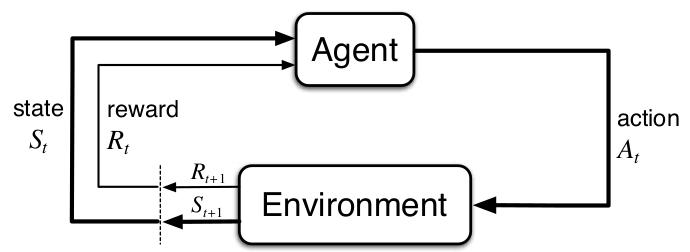
\includegraphics[width=\textwidth, height=4cm, keepaspectratio=true]{images/interaction_mdps.jpeg}
    \captionof{figure}{Agent-environment interaction in MDPs, from \cite{SuttonBarto}. \bigskip}
    \label{fig:coloring}
\end{center}

A basic yet very important premise of MDPs is that rewards only depend on the last state and action. The agent and the environment interact at a sequence of discrete time steps and, at each of them, the agent receives a static picture of the environment's state, $S_t$, and at that point it selects an action, $a_t$, given the available information. After carrying out the action, the agent receives a reward $R_t$ and finds itself at a new state $S_{t+1}$. In a finite MDP, the state, action and reward sets, $\mathcal{S}, \mathcal{A},$ and $\mathcal{R}$ respectively, are finite. In the setting of MDPs, $S_t$ and $R_t$ are random variables with discrete probability distributions that depend only on the preceding state and action. That is, for particular values of these random variables $s' \in \mathcal{S}$ and $r \in \mathcal{R}$, the probability of those values occurring at time $t$ given the values of the preceding state and action is:
\begin{equation*}
  p(s', r | s, a) \doteq Pr\{s_t = s', r_t = r | s_{t-1} = s, a_{t-1} = a\},  
\end{equation*}

for all $s', s \in \mathcal{S}, r \in \mathcal{R}$ and $a \in \mathcal{S}$. The function $p: \mathcal{S} \times \mathcal{R} \times \mathcal{S} \times \mathcal{A} \rightarrow [0, 1]$ defines the dynamics of the MDP.

Naturally, the following is true:
\begin{equation*}
    \sum_{s'\in \mathcal{S}} \sum_{r \in \mathcal{R}} p(s', r | s, a) = 1, \forall s \in \mathcal{S}, a \in \mathcal{A}.
\end{equation*}

In a Markov decision process, the probabilities given by $p$ characterize the environment dynamics completely. Moreover, the state must include all information about the past agent-environment interactions that make a difference for the future. If this is the case, then the state is said to satisfy the Markov property (\ref{markov_prop}). We assume that this property holds throughout this thesis.

From the dynamics function $p$ introduced earlier, we can obtain the \textbf{state-transition probabilities}, which we denote as $p^* : \mathcal{S} \times \mathcal{S} \times \mathcal{A} \rightarrow [0, 1]$ such that
\begin{equation*}
    p^*(s' | s, a) \doteq Pr\{s_t = s' | s_{t-1} = s, a_{t-1} = a\} = \sum_{r \in \mathcal{R}} p(s', r | s, a).
\end{equation*}

We can also compute the expected rewards given a state-action pair as $r: \mathcal{S} \times \mathcal{A} \rightarrow \mathbb{R}$ such that
\begin{equation*}
    r(s, a) \doteq \mathbb{E}[r_t | s_{t-1} = s, a_{t-1} = a] = \sum_{r \in \mathcal{R}} r \sum_{s' \in \mathcal{S}} p(s', r | s, a),
\end{equation*}

and the expected rewards given current state and action and next state as $r^* : S \times A \times S \rightarrow \mathbb{R}$ such that
\begin{equation*}
    r^*(s, a, s') \doteq \mathbb{E}[r_t | s_{t-1} = s, a_{t-1} = a, s_t = s'] = \sum_{r \in \mathcal{R}} r \dfrac{p(s', r | s, a)}{p^*(s' | s, a)}.
\end{equation*}

The MDP framework can refer to arbitrary successive stages of decision making and not necessarily to decisions made at fixed intervals of time. 

Contrary to other machine learning techniques, reinforcement learning faces the challenge known as the trade-off between exploration and exploitation. To obtain a high reward, the agent must \textit{develop a liking} for actions that it has tried in the past and have led it to good rewards so it needs to exploit what it has already experienced. However, it must also experience with other actions that can potentially mean an even higher reward, so it has to explore in order to make better action selections in the future. The dilemma here is that both exploration and exploitation strategies require the agent to fail at the task sometimes, receiving a lower reward.

A reinforcement learning agent is said to be \textbf{greedy} or to act greedily if at each state it chooses to perform the action that is believed to yield the highest reward, leaving no place for exploration. There exist several degrees of greed an algorithm can take. The greedier the algorithm, the more likely it is to converge to a sub-optimal point.

Another important reinforcement learning element is the notion of \textbf{policy}, which defines the agent's way of behaving at a given time. A policy can be thought of the sequence of actions the agent should take at every step. In some problems, the policy may be a simple function or a probability distribution over the available actions, whereas in other cases it may involve more complex computations such as a search process.

Moreover, in some reinforcement learning methods, we also have a \textbf{value function} specifying which set of actions is good in the long run. Rewards, in contrast, only determine the immediate desirability of each possible action or next state. This concept is studied in more detail in Section \ref{qlearning}.  

One way of classifying reinforcement learning methods is the following:

\begin{enumerate}[label=\roman*.]
    \item Model-free or model-based methods
    \item Policy-based or value-based methods
    \item On-policy or off-policy methods
\end{enumerate}

On the one hand, \textbf{model-based} methods build a model from the agent's understanding of the environment and such model helps predict what the next reward will be. Given the predicted reward, the agent chooses the best possible action to take. On the other hand, \textbf{model-free} methods do not build a model of the environment or reward. Instead, the agent only tries to learn the consequences of each action and maps observations to actions or to values that are related to the actions. In general, model-based methods are preferred when the problem to solve can be framed in a deterministic environment, as is the case of board games with strict rules. Model-free methods are easier to work with and are the most active area of reinforcement learning research. The two methods we present in Section \ref{implementation} and implement later on are model-free.

\textbf{Policy-based} methods directly approximate the policy of the agent. In contrast, in \textbf{value-based} methods the agent calculates the value of every possible action and chooses the action with the best outcome or value. In policy-based methods, if the policy is approximated by a deep neural network, then we are doing \textbf{deep reinforcement learning}. One of the methods presented in Section \ref{implementation} and implemented in the code is a deep reinforcement learning technique. 

\textbf{On-policy} methods evaluate and try to improve the same policy that is being used to determine which actions to take. Moreover, the agent is trained using fresh data obtained from the environment. In contrast, \textbf{off-policy} methods evaluate and try to improve another policy different from the one used to select which action to take next. In addition, the agent learns from data it has collected in previous iterations.  

Of all machine learning techniques that exist, reinforcement learning is the one that makes the most sense to use to try to find counterexamples to mathematical conjectures. This kind of problems do not come with a dataset that needs to be analyzed or for which we fit a model and obtain several predictions. Thus, one can quickly discard using supervised and usupervised machine learning techniques to refute conjectures like the ones we are trying to disprove. Instead, we need to find a way to create the data our machine learning system will ingest and it comes very natural to obtain such data from the studied conjecture in form of states and actions and generate an environment in which an agent lives. One could take, for instance, all constructions that are potential counterexamples as states and different operations one can apply to such constructions as the actions to take. In Section \ref{implementation} we study in detail how one can build an environment as well as the state and action sets for a reinforcement learning agent from graph theory conjectures.

In addition, one may want to try machine learning techniques to avoid brute force or classical search techniques when looking for counterexamples but, in the end, this is still a search problem but somehow more efficient. Moreover, for this search to be intelligent, constant feedback needs to be given to the system and this is precisely one characteristic of reinforcement learning that other machine learning paradigms do not have. 

To end this section, let us present the following diagram showing the relationship between AI and several of its subfields studied in this section. 

\begin{center}
    \centering
    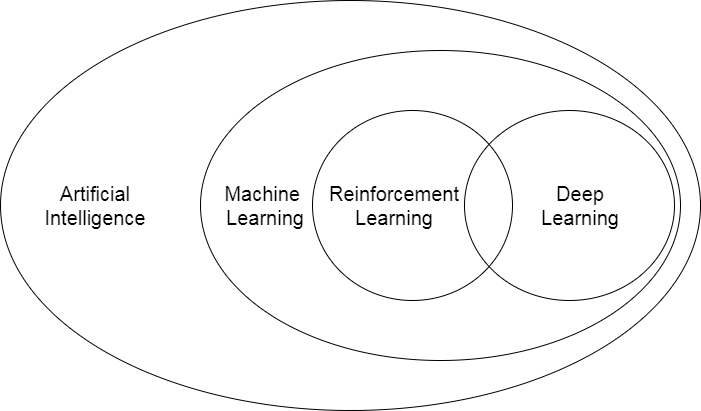
\includegraphics[width=\textwidth, height=7cm, keepaspectratio=true]{images/ai_diagram.jpeg}
    \captionof{figure}{Diagram showing the relationship between AI and several subfields, from \cite{fourati2021artificial}.}
    \label{fig:ai_diagram}
\end{center}

\newpage

% Searching Counterexamples to Graph Theory Conjectures
\section{Searching Counterexamples to Graph Theory Conjectures} \label{implementation} 

In this section we discuss how we try to search counterexamples to Conjectures \ref{wagner}, \ref{brouwer} and \ref{signless}. Let's recall that Conjecture \ref{wagner} was refuted by Wagner but we still work with it to replicate his work. We try to refute all three conjectures by using both tabular Q-learning and deep cross-entropy methods. In this chapter, we use some of the concepts introduced in Section \ref{machine learning}.

In the following subsections we discuss the reward functions given to our reinforcement learning agents and how they are derived from the conjectures as well as the implementation details for each method. We also present how the reinforcement learning environment differs between both methods, even though the underlying mechanism is the same for both of them: whether two vertices are joint via an edge is ultimately a binary decision problem. 

More about the theoretical background of the cross-entropy and the Q-learning methods as well as some useful examples and their code implementation can be found in \cite{Lapan:2020}.

\subsection{Deep Cross-Entropy Method}

The first reinforcement learning approach we take to find counterexamples to the studied conjectures is the \textbf{cross-entropy method}. Following the classification in Section \ref{reinforcement}, this method is model-free, policy-based and on-policy. In other words, this method does not build any model from the environment but rather tells the agent what to do at every state; it approximates the policy of the agent (i.e. it determines which action the agent should take at every state); and it requires new data to be obtained from the environment.

This method is quite simple from an implementation perspective and has good convergence. Moreover, it tends to work well in simple environments that do not require complex, multi-step policies or with short episodes with frequent returns, as it is our case as we will see.

During the reinforcement learning agent's lifetime, its experience is presented as \textbf{episodes} \footnote{In his work, Wagner uses the term session and number of sessions to refer to episode and batch size, respectively.} and several episodes can be grouped into a \textbf{batch} or \textbf{iteration}. Every episode corresponds to a sequence of observations the agent receives from the environment, actions it has issued and their rewards. For every episode, we calculate the total reward claimed by the agent.
This process is repeated in a loop until the episode finishes and the total reward for that episode can be calculated.

At the end of an episode, when calculating the total reward, one can decide to apply a \textbf{discount rate} $d$ to the total reward. That is, to let different rewards from one single episode have different weights in the total reward for that episode. Given a discount rate $d$, the formula for the \textbf{discount factor} for the $k$-th reward of a given episode is the following: 
\begin{equation*}
    \gamma_k = \frac{1}{(1+d)^k}.
\end{equation*}

If a given episode contains $n$ observations and $r_i$ is the reward corresponding to the $i$-th observation within that episode, then the total reward $r$ for that episode can be computed as
\begin{equation*}
    r = \sum_{i=1}^{n} \gamma_i r_i.
\end{equation*}

If the total reward is not discounted (i.e. $d=0$ and therefore $\gamma = 1$), then the total reward for an episode is just the sum of all rewards that have been computed during that episode. The larger the total reward of an episode, the better the episode from the agent's standpoint. 

Wagner does not discount the total reward in his work and neither do we in this thesis's implementation. The reason being that since the order of the edges does not matter, neither does the order the states are considered by the agent. Thus, it does not make sense to weigh the contribution of each state's reward depending on how early in an episode the agent visits such state.

Due to the way the agent selects which actions to take at each  state and to randomness in the environment, some episodes will be better than others. The core of the cross-entropy method is to discard the episodes considered bad and keep the best ones to train our model. Whether an episode is classified as good or bad depends on a boundary we set for a the total rewards of states. This boundary is a percentile of all total rewards and there is no rule of thumb to determine the optimal value of this parameter. The larger the percentile boundary, the fewer data available to train the agent. However, if the boundary is set too low we risk adding too much noise \footnote{In machine learning terminology, \textbf{noise} refers to data carrying a high proportion of irrelevant information that can mislead the model or the agent that is being trained and ultimately lead to bad results or low prediction accuracy.} and training the agent with irrelevant data. 

In our case, and following what Wagner did in his implementation, this boundary is the 93rd percentile. That is, after total reward has been calculated for all episodes, the episodes with total reward in the 93rd percentile are considered good episodes and those are the ones we want to keep. We call those episodes \textbf{elite episodes}. The episodes that do not belong to the 93rd percentile are discarded. The states and actions belonging to those elite episodes are called \textbf{elite states} and \textbf{elite actions}, respectively.

The algorithm for implementing this method can be summarized as follows: 

\begin{enumerate}
    \item An iteration starts and the environment is reset. Each iteration or batch consists of several episodes. In our code, the number of episodes within an iteration, or batch size, is set to 1,000. At each iteration, the agent interacts with the environment in the following way: 
    \begin{enumerate}[label*=\arabic*.]
        \item The agent passes an observation or state from the environment to the neural network as input and the neural network returns a probability distribution on all the possible actions from that state, with higher probability assigned to the moves that the agent thinks are best.
        \item Given these probabilities, the agent performs a random sampling to get the action that will be carried out. This allows us to add randomness to our agent as random weights make it behave in a random manner. Such randomness is especially good at the beginning of the training process since we can expect the predicted actions to be diverse enough for the agent to \textit{experiment} during the first iterations. \label{step2}
    \item Once the agent has decided which action it is going to carry out, it adds that information to the environment and obtains the next observation and the reward for the last action. 
    \end{enumerate}
    \item After all episodes in a batch have been played, we calculate the total reward for each episode and obtain the elite episodes of that batch. This reward at the end of the each session is the only feedback the neural network receives. 
    \item We train the agent with this iteration's elite episodes by passing the elite states as the input and the elite actions as the desired output. By doing this, we try to reinforce our neural network to carry out those actions that have led to good rewards.
\end{enumerate}

This process is repeated until results are good enough. At each iteration, the agent improves at selecting which action it should take at each step or state so rewards generally increase with each iteration. Typically, one may want to set a maximum number of iterations so that the method does not keep training \textit{ad infinitum}. In our implementation, the maximum number of iterations is set at 10,000, since Wagner states in \cite{Wagner:2021} that he reaches a counterexample at around iteration 5,000. Moreover, our cross entropy implementation is programmed to finish the execution if at some point a counterexample is found. In Section \ref{reward functions} we present in detail how the agent detects that a counterexample to a given conjecture has been found. 

For step \ref{step2}, we can take advantage of the fact that our problem is binary (i.e. only two actions exist). In particular, we generate only one probability and compare that value with a randomly generated number in $[0, 1]$. If the probability is larger than this random number, then we add that edge to our graph. Otherwise, we do not add that edge. We could have arbitrarily made this the other way around: add that edge to the graph if the predicted probability was lower than a random number in $[0, 1]$. 

The above information about how the algorithm to implement the cross-entropy method can be expressed in the form of pseudocode as follows: 
\begin{center}
    \centering
    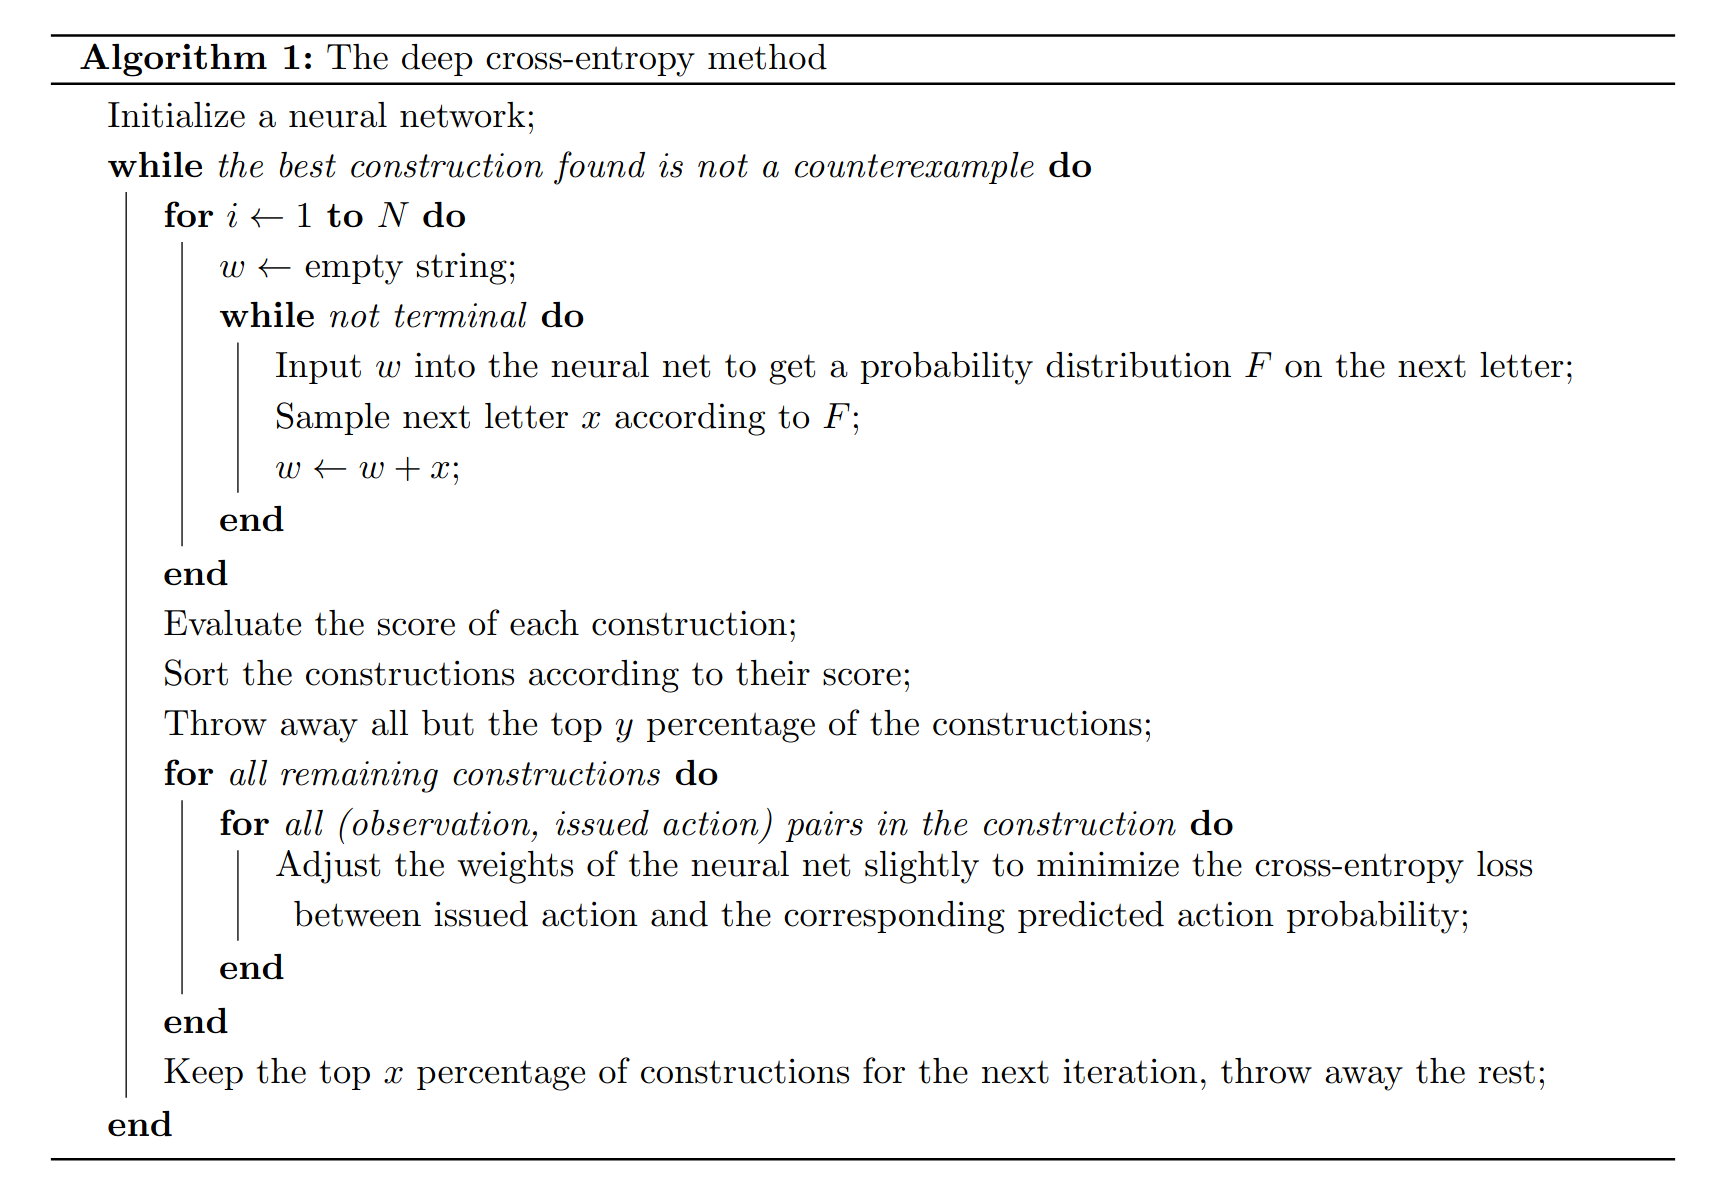
\includegraphics[width=\textwidth, height=10cm,  keepaspectratio=true]{images/pseudocode_cross-entropy.png}
    \captionof{figure}{
    Pseudocode for the deep cross-entropy method, taken from \cite{Wagner:2021}.} 
    \label{fig:pseudocode_cross-entropy}
\end{center}

% I add this pseudocode piece for this method since it is pretty confusing to follow just from the steps that I present. In my opinion, tabular Q-learning written steps are not so hard to follow so a similar pseudocode schema as this one may not be necessary

This is the approach used by Wagner in \cite{Wagner:2021} to refute Conjecture \ref{wagner}. As part of this thesis's work, we replicate what he did by defining the problem as in his paper. That is, we design our environment and derive the reward function from the conjecture in the same way as he did. The code for this thesis has been written from scratch and tries to be more straightforward and easier to follow than the original piece of code. Moreover, it uses more recent versions of several Python packages making it more robust and reproducible than Wagner's code in \cite{GithubWagner}.

The first step in designing a good reinforcement learning environment for a given problem is to encode constructions, in our case graphs, as objects the agent can work with. Since a $n$-vertex graph has at most $\frac{n(n-1)}{2}$ edges, generating a graph of $n$ vertices is equivalent to generating 0-1 sequences of length $\frac{n(n-1)}{2}$. 

From this, Wagner takes as input for the agent two vectors of length $\frac{n(n-1)}{2}$. The first vector has a 1 in all positions that correspond to edges that the agent has decided to take (i.e. to add to the graph) and a 0 in all the places the agent has rejected to add an edge to or has not considered yet. The second vector has a 0 in every position except for the one position that corresponds to the edge that is being considered at that state. 

In practice, the agent is given all this information in one single vector of length $n(n-1)$. Every instance of this 0-1 array of length $n(n-1)$ represents the state that we are in and it is the input the agent receives. The 0-1 encoding makes plenty of sense here since at each state, the agent has two possible actions: adding the edge it is considering at that state or not. 

In our implementation, the policy is approximated by a deep neural network so we are actually implementing the deep version of the cross-entropy method, i.e. the \textbf{deep cross-entropy method}. Such neural network only learns to predict the optimal move at each state, it does not learn a value function for the states or the state-action pairs.

As for the deep neural network that approximates the policy, we use the same specification as Wagner and it has three hidden layers with 128, 64 and 4 neurons, respectively. We use the binary cross-entropy loss function as we predict a binary outcome. The chosen optimizer is stochastic gradient descent optimizer with a learning rate set at 0.0001 which is a value that, according to Wagner's research, reaches a balance between the speed of convergence and preventing the agent to get stuck in suboptimal constructions.

\subsection{Tabular Q-Learning} \label{qlearning}

The second reinforcement learning approach we take to try to find counterexamples to graph theory conjectures is Q-learning. And, in particular, \textbf{tabular Q-learning}, a model-free, policy-based and off-policy method. Q-learning is an old family of algorithms but it deserves its own place in this thesis as it was the first algorithm with guaranteed convergence to the optimal policy, see \cite{watkins:dayan}. It was originally proposed by Watkins in \cite{watkins}.

Before entering into how this method works and how we can implement it, we need to present the value iteration method.

We first define the \textbf{value of a state} as the expected total reward that is attainable from the state. Formally, the value of state $s$ can be defined as
\begin{equation*}
    V_s = \mathbb{E} \big[ \sum_{t=0}^{\infty} r_t \gamma^t],
\end{equation*}

where $r_t$ is the local reward obtained at step $t$ and $\gamma$ is the discount factor as defined earlier. 

The following graph showing an abstract environment can make it easier to visualize the notions that we are about to introduce: 

\begin{center}
    \centering
    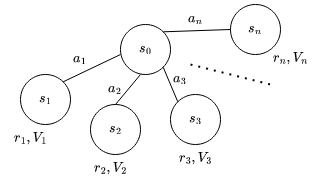
\includegraphics[width=\textwidth, height=4.5cm, keepaspectratio=true]{images/deterministic_env.png}
    \captionof{figure}{
    Example of an abstract deterministic environment.} 
    \label{fig:det_env}
\end{center}

Let us assume that our agent lives in a deterministic environment, where all actions have a guaranteed outcome. Suppose the agent observes state $s_0$ which has $n$ available actions. Every action leads to another state $s_1, ..., s_n$ with respective reward $r_1, ..., r_n$. Further, assume that we know the values $V_1, ..., V_n$ of all states connected to $s_0$. Throughout this section we denote the state set, action set and rewards set as $\mathcal{S}, \mathcal{A}$ and $\mathcal{R}$, respectively. To determine the action it should take, the agent needs to calculate the resulting values of each action and choose the action that yields the maximum value. That is, it calculates the following:
\begin{equation} \label{bellman}
    V_0 = \max_{a_i \in \mathcal{A}}(r_i + \gamma V_i),
\end{equation}

where $V_i$ refers to the value of the next state and is a measure of the long-term value of the state $s_0$ and $A$ is the set of all available actions from $s_0$.

By adding the (discounted) value of the next state, $V_i$, to the above expression, the agent is discouraged to act greedily so it gets to better possible outcomes than if it just looked at each action's reward. Equation \ref{bellman} is the \textbf{Bellman equation} (of value). The Bellman Equation determines the maximum reward an agent can receive if it makes the optimal decision at the current state and at all following states. Further, it recursively defines the value of the current state as the maximum possible value of the current state reward plus the (discounted) value of the next state. The Bellman equation gets its name from Richard Bellman who, in fact, coined the term \textit{dynamic programming}.

This same idea can be extended to a stochastic scenario or environment, when a given action can lead the agent to different states with different probabilities. The following diagram exemplifies this case.

\begin{center}
    \centering
    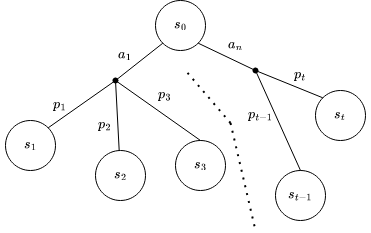
\includegraphics[width=\textwidth, height=4.5cm, keepaspectratio=true]{images/stochastic_env.png}
    \captionof{figure}{
    Example of an abstract stochastic environment.} 
    \label{fig:stoch_env}
\end{center}

Formally, in a stochastic environment, the expected value after carrying out action $a_i$ from $s_0$ is calculated in the following manner:
\begin{equation*}
    V_0(a_i) = \mathbb{E}_{s\sim \mathcal{S}}[r_{s,a_i} + \gamma V_i] = \sum_{s \in \mathcal{S}} p_{a_i, 0 \rightarrow s} (r_{s, a_i} + \gamma V_i),
\end{equation*}

where $p_{a_i, j \rightarrow k}$ refers to the probability of action $a$ issued in state $j$ leading to state $k$.

If we combine Equation \ref{bellman} for the deterministic case with the value in stochastic environments, one can get the generalized Bellman equation: 

\begin{equation} \label{bellman generalized}
    V_0(a_i) = \max_{a_i \in \mathcal{A}} \mathbb{E}_{s\sim \mathcal{S}}[r_{s,a_i} + \gamma V_i] = \max_{a_i \in \mathcal{A}} \sum_{s \in \mathcal{S}} p_{a_i, 0 \rightarrow s} (r_{s, a_i} + \gamma V_i).
\end{equation}

Thanks to Equation \ref{bellman generalized}, any agent can obtain at each state the optimal policy to obtain a given reward. Moreover, if it knows the value for every state, then it automatically knows how to get the maximum reward.

Another very important concept related to the value of state $s$, $V_s$, is the \textbf{value of an action} $a$ at state $s$, denoted as $Q_{s, a}$. It can be thought of the total reward one can get by executing action $a$ at state $s$. 

We want to get values of $Q$, also known as \textbf{Q-values}, for every pair $\{s, a\}$. $Q$ for state $s$ and action $a$ is just the expected immediate reward and the (discounted) long-term reward of the next state $s'$. Thus, one has

\begin{equation} \label{qvalues}
    Q_{s, a} = \mathbb{E}_{s' \sim \mathcal{S}} [r_{s, a} + \gamma V_ {s'}] = \sum_{s' \in \mathcal{S}} p_{a, s \rightarrow s'} (r_{s, a} + \gamma V_{s'}).
\end{equation}

Equation \ref{qvalues} can be expressed recursively as 
\begin{equation*}
    Q_{s, a} = r_{s, a} + \gamma \max_{a' \in \mathcal{A}} Q_{s', a'}.
\end{equation*}

Moreover, it is true that the value of state $s$ equals the value of the best action we can execute from state $s$ as:
\begin{equation*}
    V_s = \max_{a \in \mathcal{A}} Q_{s, a}.
\end{equation*}

From an agent's point of view it is more convenient to work with Q-values than with the values for the states since to choose the optimal action at one given state using the Q-values the agent just needs to compute $Q$ for all available actions using the current state and execute the action with the largest value of $Q$. In contrast, to choose the best action using the values of the states the agent needs to know values and probabilities for transitions, which is something unknown in advance by the agent and it would have to estimate them.

The \textbf{value iteration method} is an algorithm that allows to numerically calculate the values of the states and values of the actions of Markov decision processes with known transition 
probabilities and rewards. This algorithm for the state values consists of the following steps: 

\begin{enumerate}
    \item Initialize the values of all states to some initial value which is usually 0.
    \item For every state $s$ in the MDP, perform the following Bellman update: 
        \begin{equation*}
            V_s \leftarrow \max_a \sum_{s'} p_{a, s \rightarrow s'} (r_{s, a} + \gamma V_{s'}).
        \end{equation*}
    \item Repeat step 2 for some large number of states or until changes become very small.
\end{enumerate}

In the case of action values given a state, that is, $Q_{s, a}$, the steps to take are: 
\begin{enumerate}
    \item Initialize every $Q_{s, a}$.
    \item For every state $s$ and action $a$ in this state update $Q_{s, a}$ in the following way:
        \begin{equation*}
            Q_{s, a} \leftarrow \sum_{s'} p_{a, s \rightarrow s'} (r_{s, a} + \gamma \max_{a'} Q_{s, a})
        \end{equation*}
    \item Repeat step 2 for some large number of states or until changes become very small.
\end{enumerate}

However, it is not really necessary to iterate over every state in the state space as we can design an environment that can anticipate what would happen at each possible next state given the current state and all possible actions to execute from it. This modification of the value iteration method is called Q-learning. In particular, since the Q-values $Q_{s, a}$ are stored in a table, the presented algorithm is actually called \textbf{tabular Q-learning} and it consists of the following steps:

\begin{enumerate}
    \item Initialize a table that maps states to values of actions. We denote the elements of this table as $Q_{s, a}$. \label{step1}
    \item Interact with the environment and obtain $(s, a, r, s')$, a tuple containing the current state, the action the agent should take, the reward and the next state. 
    \item Update the table with the value for this state and best action using the Bellman approximation. Moreover, to prevent the training process from becoming unstable one may want to keep some information about previous values of $Q_{s, a}$. For this reason, we use what is known as a blending technique that computes a weighted average between old and new values of $Q_{s, a}$ using a learning rate $\alpha \in [0, 1]$. Thus, the update looks like: 
    \begin{equation*}
        Q_{s, a} \leftarrow (1 - \alpha)Q_{s, a} + \alpha \big( r + \gamma \max_{a' \in \mathcal{A}} Q_{s', a'} \big).
    \end{equation*}
    \item Check convergence conditions. If they are not met, we repeat from step 2. \label{conv}
\end{enumerate}

As for step \ref{step1}, in our implementation we initialize our Q-table with random  integer numbers in [0, 10]. This allows us to add a bit of randomness at the beginning of the training process for our agent.

In step \ref{conv}, to check if the agent is converging to a solution, one can simply study if the current solution has not changed much with respect to the previous one. One way of doing so is by defining a convergence function such as: 
\begin{equation*}
    c(Q_{s, a}, Q_{s', a'}, \epsilon) = \begin{cases} 1, & \text{if }  |Q_{s, a} - Q_{s', a'}| < \epsilon, \forall s \in \mathcal{S}, \forall a \in \mathcal{A} \\ 0, & \text{otherwise} \end{cases},
\end{equation*}

where $\epsilon$ is a tolerance parameter that can be arbitrarily set at a very close to 0 but positive value. One must note that this criterion does not guarantee that the reinforcement learning algorithm converges to the global optimal value function but to some local optimal value function.  

In our implementation, instead of relying on a convergence function, we arbitrarily set a maximum number of iterations, 10,000, so that the execution stops if no counterexample has been found and the 10,000th iteration is reached. As in the deep cross-entropy implementation, the executions stops if a counterexample is found.

In contrast to the environment for the deep-cross entropy method, the environment now only consists of an array with all possible actions (i.e. 0 and 1, not joining two vertices and joining them, respectively) and a $\frac{n(n-1)}{2}$ 0-1 vector representing all potential edges of a graph. These two arrays are all we need to be able to generate and initialize the Q-table.

As already mentioned, Q-learning solves the issue of iterating over the full set of states. Nonetheless, this approach may not be optimal when the state set is very large, which is something that may happen as larger graphs are considered. For such cases, one can use a non-linear representation to map each state and action pair to a value instead of a table. In the realm of machine learning, this problem is just a regression problem. The optimal specification for this regression function will depend on each particular problem. 

Nonetheless, one common approach is to use a deep neural network to map each state and action to a value. When that is the case, the method becomes \textbf{deep Q-learning} and it suffers a few modifications. First, we go back to work with batches of episodes to train the neural network. As we have already seen, the size of a batch of episodes is variable and it is at the end of the episode that we give feedback to our neural network. 

The algorithm for the deep Q-learning implementation consists of the following steps: 

\begin{enumerate}
    \item Initialize $Q_{s, a}$ with some initial approximation.
    \item Obtain the tuple $(s, a, r, s')$ from interacting with the environment. 
    \item Calculate the loss function: 
    \begin{itemize}[label=\raisebox{0.25ex}{\tiny$\bullet$}]
        \item $\mathcal{L} = (Q_{s, a}  - r)^2$ if the episode has ended, and
        \item $\mathcal{L} = \Big(Q_{s, a}  - (r + \gamma \max_{a' \in A} Q_{s, a}) \Big)^2$ otherwise.
    \end{itemize}
    \item Update $Q_{s, a}$ using the deep neural network specification of choice with the loss function as defined above. 
    \item Check convergence conditions. If they are not met, repeat from step 2.
\end{enumerate}

The target or response variable for the function approximated by the neural network are the $Q_{s, a}$ values obtained using the Bellman equation. However, a practical issue with the default training procedure for deep Q-learning is the lack of independent data. Since $s$ and $s'$ have only one step between them, it is very difficult for a neural network to distinguish between them and the assumption of i.i.d data is violated. 

There are several techniques that help solve this issue, one of them being the so-called replay buffer that yields quasi-independent data. The specific details of these techniques as well as their implementation are beyond the scope of this thesis and we are not using deep Q-learning for our counterexample search. However, one can read about this method in Chapter 6 from \cite{Lapan:2020}.

\subsection{Reward Functions} \label{reward functions}

As mentioned in Section \ref{reinforcement}, the reinforcement learning agent tries to maximize the so-called reward function. The choice of such function depends on the problem that is trying to be solved. In our case, each reward function can be derived from the conjecture we are trying to disprove.

In Conjecture \ref{wagner}, we have the following expression:
\begin{equation*}
    \lambda^*(G) + \mu(G) \geq \sqrt{n-1} +1, 
\end{equation*}

where $\lambda^*(G)$ is the largest eigenvalue of a connected graph $G$ of $n \geq 3$ vertices and $\mu(G)$ is its matching number.

This expression can be rearranged to obtain the following:

\begin{equation} \label{reward function wagner}
    \sqrt{n-1} + 1 - (\lambda^*(G) + \mu(G)) \leq 0.
\end{equation}

When a given graph has $\lambda^*(G), \mu(G)$ and $n$ such that Expression (\ref{reward function wagner}) is not satisfied, i.e $\sqrt{n-1} + 1 - (\lambda^*(G) + \mu(G)) > 0$, then we have found a counterexample. Therefore, we take 
\begin{equation} \label{r1}
    r_1(G) = \sqrt{n-1} + 1 - \big(\lambda^*(G) + \mu(G)\big)
\end{equation}
as the reward function for Conjecture \ref{wagner} so this is what our reinforcement learning agent will want to keep maximizing until it crosses the 0 cut-off point. 

From Conjectures \ref{brouwer} and \ref{signless}, we have

\begin{equation} \label{reward function brouwer}
    \sum_{i=1}^{t} \lambda_i(G) \leq e(G) + {t+1 \choose 2}
\end{equation}

as restriction.

Similarly, from Expression (\ref{reward function brouwer}) we can obtain that if for any $t \in \{1,\ldots, n\}$

\begin{equation*}
    r_t(G) = \sum_{i=1}^{t} \lambda_i(G) - e(G) - {t+1 \choose 2}
\end{equation*}

is strictly positive, then we have found a counterexample. Therefore, one may naturally think that $r_t(G)$ can be good candidates for the reward function for Conjectures \ref{brouwer} and \ref{signless}. However, if that was the case, we would have several reward functions associated to one single graph and that would confuse our system. Since that cannot be the case, we take

\begin{equation*}
    r_2(G) = \max_t r_t(G) = \max_t \Big( \sum_{i=1}^{t} \lambda_i(G) - e(G) - {t+1 \choose 2} \Big)
\end{equation*}

as the reward function for Conjectures \ref{brouwer} and \ref{signless}.

\subsection{Constraints of Learning-Powered Counterexample Search} \label{constraints}

% MOURE AIXO DINS DAQUESTA SECCIO ON MILLOR CONVINGUI
%

Up until now, this thesis has presented some reinforcement learning methods that can help find counterexamples to refute graph theory conjectures. This section explores the necessary conditions for these  methods or any other reinforcement learning techniques to be applied. Moreover, we justify that Conjectures \ref{wagner}, \ref{brouwer} and \ref{signless} satisfy those conditions.

As we have seen, the first step when building a reinforcement learning agent to find counterexamples is to translate the conjecture into a language or code the computer can understand and to derive a reward function from the studied conjecture. Therefore, the first important requirement to be fulfilled is to have a conjecture from which a function to be optimized can be derived. 

Further, we need the conjecture to be translated to a problem that is not too complex for a computer to solve, i.e. the problem needs to be computationally efficient. The \textbf{complexity} of a given optimization problem is a measure of how difficult it is to solve. In a sense, computational complexity is related to the amount of resources (including time) consumed by a computer while performing a given task. One can read about computational complexity in \cite{AroraBarak, Burgisser}.

The \textbf{P class} consists of all decision problems (i.e. problems with a "yes" or "no" answer) that can be solved in polynomial time $\mathcal{O}(n^k)$. That is, problems that can be solved in less than $cn^k$ steps, where $c$ and $k$ are constants independent from the input size $n$. An example of a problem belonging to the P complexity class is deciding whether a graph has an Eulerian tour. Problems belonging to the P class are referred to as \textit{efficiently computable} problems.

The decision problem of our agent to compute the reward of all possible actions at each state must belong to the P complexity class. Otherwise, the agent may never be able to learn an acceptable policy. 

Further, the reward function must be evaluated at each step. In other words, it cannot be the case that for a given construction that is a potential counterexample the function is not defined. 

In Section \ref{reward functions} we have derived three reward functions from three different spectral graph theory conjectures. 
We know that one can efficiently compute the eigenvalues of a matrix \cite{qr_algorithm} and the matching number of a graph \cite{matching_efficient}. Therefore, we can evaluate all reward functions at all states. Thus, we state that this first condition for using reinforcement learning is satisfied for all three conjectures we are trying to disprove.

The second necessary condition for reinforcement learning to be applied has not been found in the literature in a formal manner. In consequence, here we attempt to formally introduce a second restriction for reward functions derived from graph theory conjectures. However, we first need to introduce some concepts. 

A reward function is said to be \textbf{sparse} if it is zero in most of its domain. A sparse reward function gives insufficient feedback to the agent about whether an action yield to a relative reward at a given state. In contrast, a \textbf{dense} reward function assigns a non-zero value to most of the transactions, allowing the agent to receive feedback at almost every step.

Naturally, learning in environments with sparse reward functions is much more challenging than with dense reward functions since the agent receives fewer data points as feedback compared to the dense reward case. In fact, most reinforcement learning methods with a sparse reward function fail to learn an acceptable policy in a reasonable time frame \cite{sparse}. Thus, we want our problem to have dense reward functions. 

We can go one step further and not only impose that our reward function must be dense but that we want our reward set, i.e. the range of our reward function, to be as large as possible, to avoid our agent taking too long to learn a decent policy. In other words, we want high variability in the values taken by the reward function. Formally, we try to express this as follows. Let $r: \mathcal{G}_n \rightarrow \mathbb{R}$ be a real-valued reward function with $\mathcal{G}_n$ being all the graphs of $n$ vertices (that are considered by our algorithm). Then, the reward function $r$ must satisfy that $\exists c \text{ } \forall S \subseteq r(\mathcal{G}_n)$ such that $|r^{-1}(S)| \leq c|S|$, with $c$ being much smaller than $|\mathcal{G}_n|$. One can see whether this condition holds by observing the reward values after just a few iterations. In our case, all three conjectures satisfy this condition.

%The \textit{NP class} consists of all decision problems that can be efficiently \textbf{verified} (but not necessarily solved) in deterministic polynomial time. In this context, to verify means to ensure a solution is correct by checking that it satisfies any and all equations and/or inequalities in a problem. Note that by definition P $\subseteq$ NP. However, it is unknown whether NP $\subseteq$ P holds. Given a list of n numbers $A_1,...,A_n$ and a number $T$, deciding whether there is a subset of the numbers that sums up to $T$ belongs to the NP class. Another problem belonging to this class is deciding whether a given graph has a Hamiltonian cycle\footnote{See Definition \ref{Hamiltonian cycle} for a definition of Hamiltonian cycle.}.

%A problem is said to be \textit{NP-hard} if it is at least as hard as any other problem belonging to the NP class. The \textit{NP-hard class} is the collection of all NP-hard problems.

%Given two problems $A$ and $B$, $A$ is \textit{reducible} to $B$ if an algorithm for solving $B$ efficiently (assuming it exists) can also be used as a subroutine to solve $A$ efficiently. 

%A problem is said to be \textit{NP-complete} if it belongs to the NP class and all other NP problems are reducible to this problem. NP-complete problems lie at the intersection between NP and NP-hard problems. The \textit{NP-complete class} consists of all NP-complete problems.

%The \textbf{P vs. NP problem} is a major unsolved problem in mathematical logic and theoretical computer science. It is unknown whether P $=$ NP actually holds. If that were the case, every problem the solution of which could be verified in an efficient manner could also be efficiently solved. 

%The notions presented in this section can be summarized in the following way depending on the outcome of the P vs. NP problem. \newline

%\begin{center}
    %\centering
    %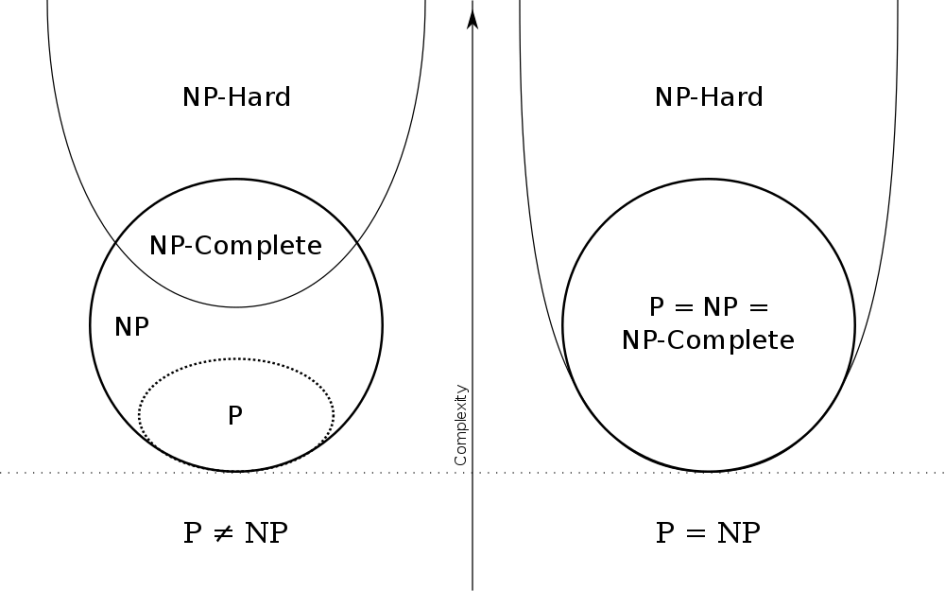
\includegraphics[width=\textwidth, height=5cm, keepaspectratio=true]{images/p_vs_np.png}
    %\captionof{figure}{
    %Complexity classes as sets and subsets depending on whether P=NP holds, from \cite{PvsNP:2017}.
    %} 
    %\label{fig:PvsNP}
%\end{center}

%At this point, one may quickly realize that the \textit{computational efficiency} that was listed as a requirement at the beginning of the section actually means that the optimization problem the reinforcement learning agent will need to solve must belong to the P complexity class. Therefore, when translating a counterexample to an environment that can be understood and potentially solved by an agent, one must always design such environment in a way that the reward function optimization problem can be solved in polynomial time.

\subsection{Code Implementation}

\subsubsection{Some Notes about our Implementation}

Wagner notes in \cite{Wagner:2021} that Conjecture \ref{wagner} appears to be true for graphs of $n \leq 18$ vertices. He implements the cross entropy method for $n=19$ and finds a counterexample of that size. We do the same and implement both deep cross-entropy and tabular Q-learning methods with the number of vertices of our graphs set to 19. 

As for Conjecture \ref{brouwer}, we know it is true for graphs of $n \leq 10$ vertices. Therefore, we implement both methods for graphs with $n\in [11, 20]$ vertices. For Conjecture \ref{signless}, we implement both methods for graphs with $n \in [11, 20]$ as well since the authors of \cite{Ashraf:Omidi:Tayfeh-Rezaie} check by computation the conjecture holds for all graphs up to 10 vertices.  

To discourage the reinforcement learning agent from carrying out a specific action (i.e. take as a potential counterexample a graph for which we know a conjecture is true), we can assign to that specific graph's reward function value a \textbf{maximum penalty}. In our case, we want this maximum penalty to be a very large negative number as we want to ultimately find our way to a positive reward function value when a counterexample exists. 

The value of the maximum penalty is $- \infty$ for the deep cross-entropy method and $- 100,000$ for the tabular Q-learning method. The value of $- 100,000$ is an arbitrarily large (in magnitude) negative number since we cannot use $- \infty$ in this setting. Let us recall that Q-values are computed using recursive addition and that the values of the reward function are ultimately involved in that sum. Thus, if the reward function takes at some point the value of $- \infty$, then all Q-values will be $- \infty$ as well, which does not help our agent decide which action is better to take.

When trying to refute Conjecture \ref{wagner} we assign the maximum penalty to all unconnected graphs since the conjecture only takes into consideration graphs that are connected. As for Conjecture \ref{brouwer}, the maximum penalty is assigned to graphs for which this conjecture is known to be true, as listed in Section \ref{subsection conjectures}. Finally, for Conjecture \ref{signless} we assign the maximum penalty to regular graphs and trees as it has been proved to be true for these graphs.

\subsubsection{Programming Language and Framework}

Python is the default programming language used in machine learning research and applications. This comes as no surprise since it has a very simple syntax that makes it very intuitive and easy to learn. It is also open-source and therefore accessible to everyone. Moreover, it has an active community that is constantly developing new libraries and maintaining existing ones. 

The code runs on Python 3.7 to guarantee compatibility with the chosen cloud computing services, which are discussed in the next subsection. However, it can also be run on more recent versions of Python, even though it is possible that some libraries may need to be updated. 

When developing machine learning applications, one may want to use existing frameworks that make the entire process of building and training neural networks faster and easier. There exist several frameworks that work with Python but the one we use for our implementation is TensorFlow \cite{tensorflow}. The way we interact with TensorFlow is via Keras \cite{chollet2015keras}, a TensorFlow wrapper. This basically means that when we call a Keras function this in turn calls a sequence of TensorFlow functions. 

For dealing with graph constructions and performing operations on graphs, the NetworkX library \cite{hagberg2008exploring} is of great help. Moreover, in our code we use some functions from the Scipy \cite{2020SciPy-NMeth} and Numpy \cite{harris2020array} libraries, two of the most common Python libraries that are useful for scientific and advanced computing. 

Furthermore, we have used the Logtail \cite{logtail} and Psutil \cite{psutil} libraries to manage logs written by our code to detect any problems and to keep track of the memory allocation during the execution of the deep cross-entropy method, respectively.

\subsubsection{Using Cloud Services for Remote Execution}

Due to the large load of computer power needed to execute the deep cross-entropy to try to disprove Conjectures \ref{wagner}, \ref{brouwer} and \ref{signless}, one is better-off looking for alternatives to the local execution of the scripts. There exist multiple cloud computing services providers and it is very accessible and affordable for an individual developer to use such services for their own projects. 

For this thesis's code implementation we have used Amazon Web Services, AWS for short, to execute our code in the cloud. The AWS service we have worked with is Elastic Cloud Computing, EC2 for short. In particular, we have used EC2 spot instances, a type of instance that uses spare EC2 capacity and that is available for less than the price for regular on-demand instances. The instance type used is g4dn.xlarge, one of the available GPU-based instances. In \cite{ec2} one can find more about AWS EC2.

To create, manage and terminate the instances in a simplified manner we have used Spotty, a tool to train machine learning models in AWS or Google Cloud. More about this Python library in \cite{spotty}.

\subsubsection{Problems Encountered During the Execution}

During the remote execution of the deep cross-entropy method the machine was running out of RAM due to an identified issue in Keras by several users \cite{memory_leak}, preventing us to get past the 380th iteration. The same would happen when trying to run the code locally. Wagner found this same problem, as he notes in the first few commented lines in his script \cite{wagner_code} and he solved it downgrading to older versions of both Python and TensorFlow. However, when we tried to do the same Wagner did in 2021, we encountered that those older versions were not supported anymore and our code was not able to run. 

Finally, after doing some research, we discovered that in our version of Keras there exists a specific function that can remove unnecessary information automatically stored that takes up a lot of RAM without compromising the trained model. After implementing this, our deep cross-entropy code was able to run smoothly without any memory leaks.

\subsection{Discussion of Results}

Unfortunately, after running both the deep cross-entropy and Q-learning methods for Conjectures \ref{wagner}, \ref{brouwer} and \ref{signless} we have not been able to find any counterexample to any of these conjectures. Nonetheless, we use this section to discuss why this may have been the case and present the counterexample found by Wagner and presented in his paper \cite{Wagner:2021}. 

We know Conjecture \ref{wagner} is false and since we have replicated Wagner's approach, we were expecting we would reach a counterexample using the deep cross-entropy method. Nonetheless this has not been the case and we suspect the reason is that 10,000 iterations were not enough for our agent, even though they were enough for Wagner. 

The following figure shows the counterexample Wagner found. It is a 19-vertex tree with largest eigenvalue $\sqrt{10}$ and matching number 2.

\begin{center}
    \centering
    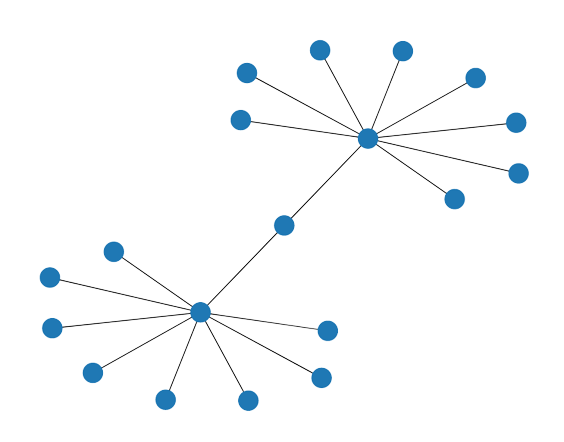
\includegraphics[width=\textwidth, height=4cm, keepaspectratio=true]{images/counterexample_wagner.png}
    \captionof{figure}{19-vertex graph that does not satisfy Conjecture \ref{wagner}, from \cite{Wagner:2021}.}
    \label{fig:wagner_counterexample}
\end{center}

Wagner notes in \cite{Wagner:2021} that trees are the best counterexample candidates for Conjecture \ref{wagner} since for a graph $G$ with largest matching $M$, one can repeatedly delete edges from $E(G)\setminus M$ without disconnecting the graph. One can do this without changing $\mu(G)$, but the value of the largest eigenvalue decreases.

We suspect the reason Q-learning has not led us to a counterexample for Conjecture \ref{wagner} is also the fact that we did not allow the agent run for enough iterations. Another potential cause is how the states have been defined, where the agent does not know the difference between an edge taking the value of 0 because it has deliberately chosen not to join those two vertices or because that edge has not been visited yet. 

As for Conjecture \ref{brouwer}, Brouwer's conjecture, we were not expecting any counterexample to be found since it is most likely a true statement, even though no one has been able to derive a formal proof yet. Moreover, in \cite{Rocha:2019} the author shows that for a sequence of random graphs Brouwer’s conjecture holds true with probability tending to 1 as the number of vertices tends to infinity. Thus, if a counterexample to that conjecture exists, it is very difficult to find. In contrast, Conjecture \ref{signless} is probably a bit more likely to be false that Conjecture \ref{brouwer}. However, since it has been proven true for some types of graph, finding a counterexample to it is not an easy task either.

\newpage

% Conclusions and Further Work
\section{Conclusions and Further Work} \label{conclusions}

In this thesis we have reviewed some graph theory concepts and presented some graph theory conjectures with the aim of refuting them. The thesis has focused on how machine learning and, in particular, reinforcement learning can be a part of a mathematics researcher's toolbox to find counterexamples to conjectures. Despite the fact that there does not exist a lot of literature about using reinforcement learning to refute conjectures, one can expect that in the coming years more and more researchers will publish results after using these methods. Further, new algorithms are still to be created and it is possible that with time there will be a reinforcement learning method specifically designed and optimized to look for counterexamples to graph theory conjectures. 

We have also presented the results obtained by Wagner in \cite{Wagner:2021} after applying the deep cross-entropy method to refute Conjecture \ref{wagner}. This is so far the first known case of a counterexample being found by a reinforcement learning agent in the literature, even though a counterexample had previousy been found to this conjecture by Stevanović \cite{zbMATH05804421}.

We have implemented the deep cross-entropy and tabular Q-learning methods, two reinforcement learning techniques, to try to refute Conjectures \ref{wagner}, \ref{brouwer} and \ref{signless}. Nonetheless, after a successful implementation, we have not been able to obtain any counterexample to any of the studied conjectures. 

After the lack of successful results we can, however, present some work that could be further done related to what this thesis has focused on.

\begin{enumerate}[label=\roman*.]
    \item Re-run the deep cross-entropy and tabular Q-learning methods allowing for a larger number of maximum iterations. 
    \item Redesign the state architecture for the tabular Q-learning method so the agent can distinguish between the edges that have been discarded in previous iterations and the ones which have not been considered yet. 
    \item Initialize the Q-tables with random integers using ranges different from $[0, 10]$, as this may require a bit of experimentation.
    \item Closely monitor the behavior of the agent by studying whether its preferred constructions share any characteristics (i.e. they are all trees or the value of a given invariant coincides) as we approach the maximum number of iterations.
    \item Try to refute the same conjectures by implementing more sophisticated algorithms such as deep Q-learning.
\end{enumerate}

\newpage
\renewcommand{\thepage}{}

% Bibliography and References
\nocite{*}
\bibliography{biblio.bib}
\bibliographystyle{ieeetr}  

\newpage

% Appendix

%\section{ChatGPT as a Proof-Assistant} \label{apx:chatgpt}
%The \textbf{five color theorem} states that every planar graph has a vertex of degree at most 5. After asking ChatGPT to prove this theorem for us this was what it yielded: \kolja{note that this is NOT a correct proof}
%\begin{center}
    %\centering
    %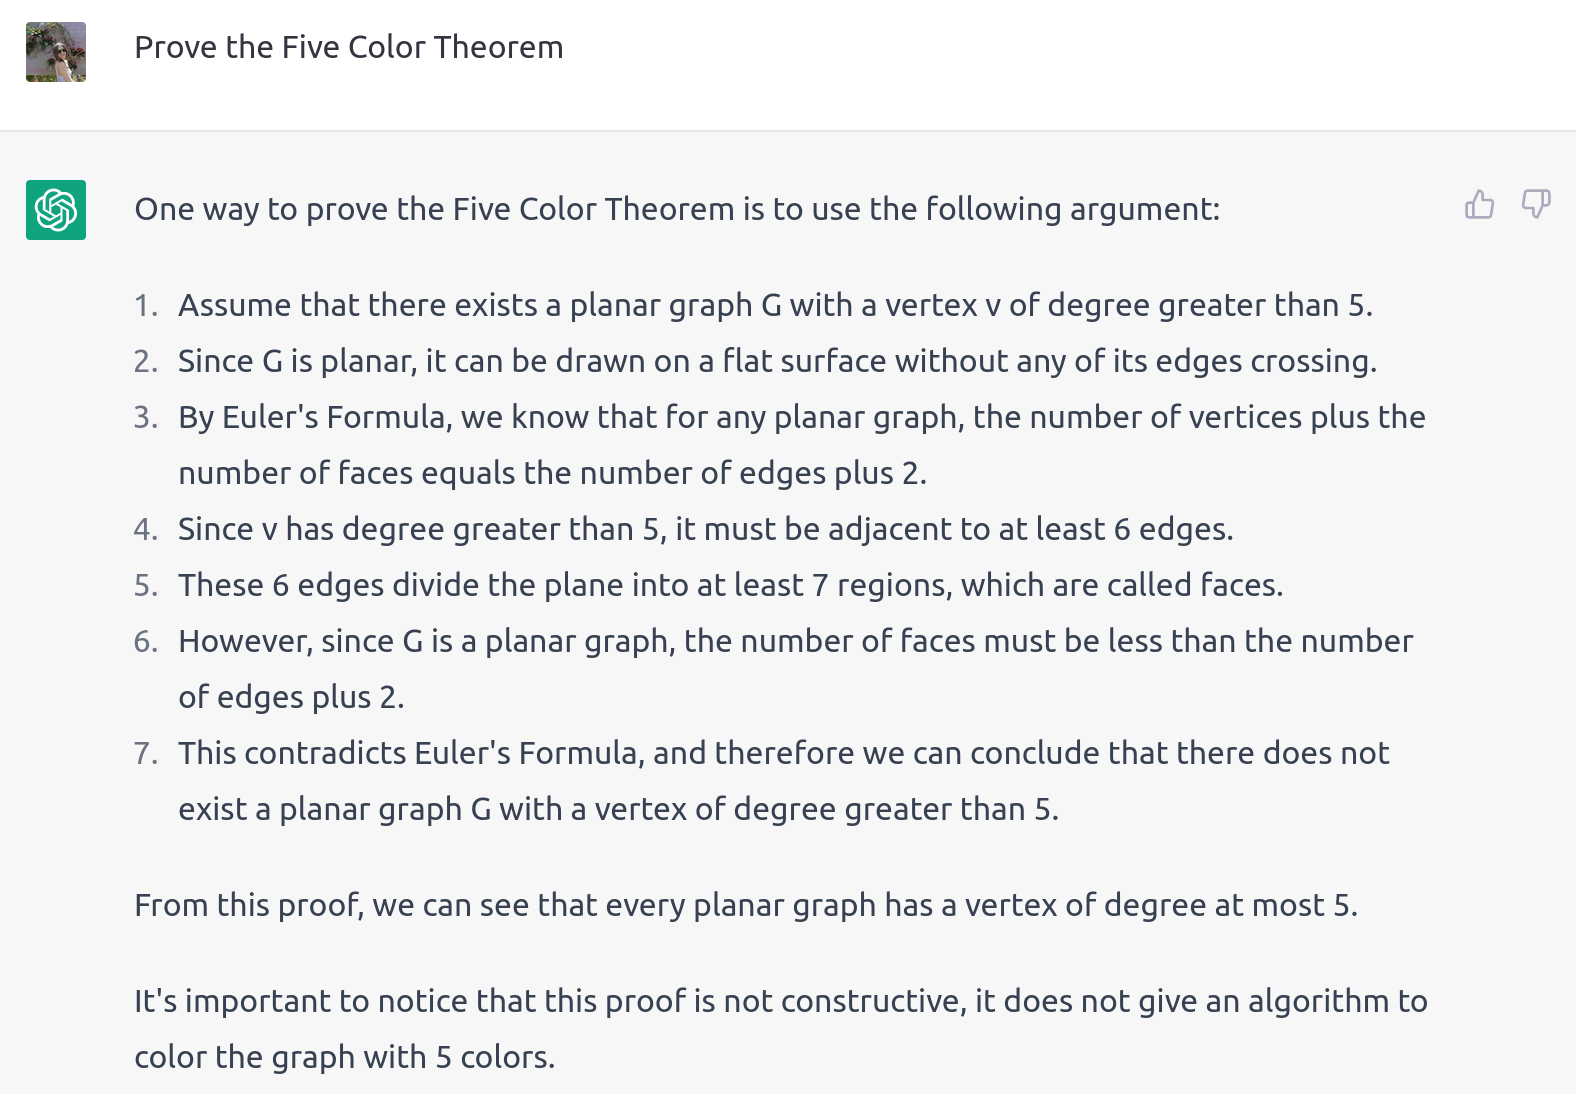
\includegraphics[width=\textwidth, height=12cm, keepaspectratio=true]{images/chatgpt2.png}
    %\label{fig:chatgpt}
%\end{center}

\appendix

\section{Neural Network Activation Functions} \label{apx:activation}
\bigskip
\begin{center}
    \centering
    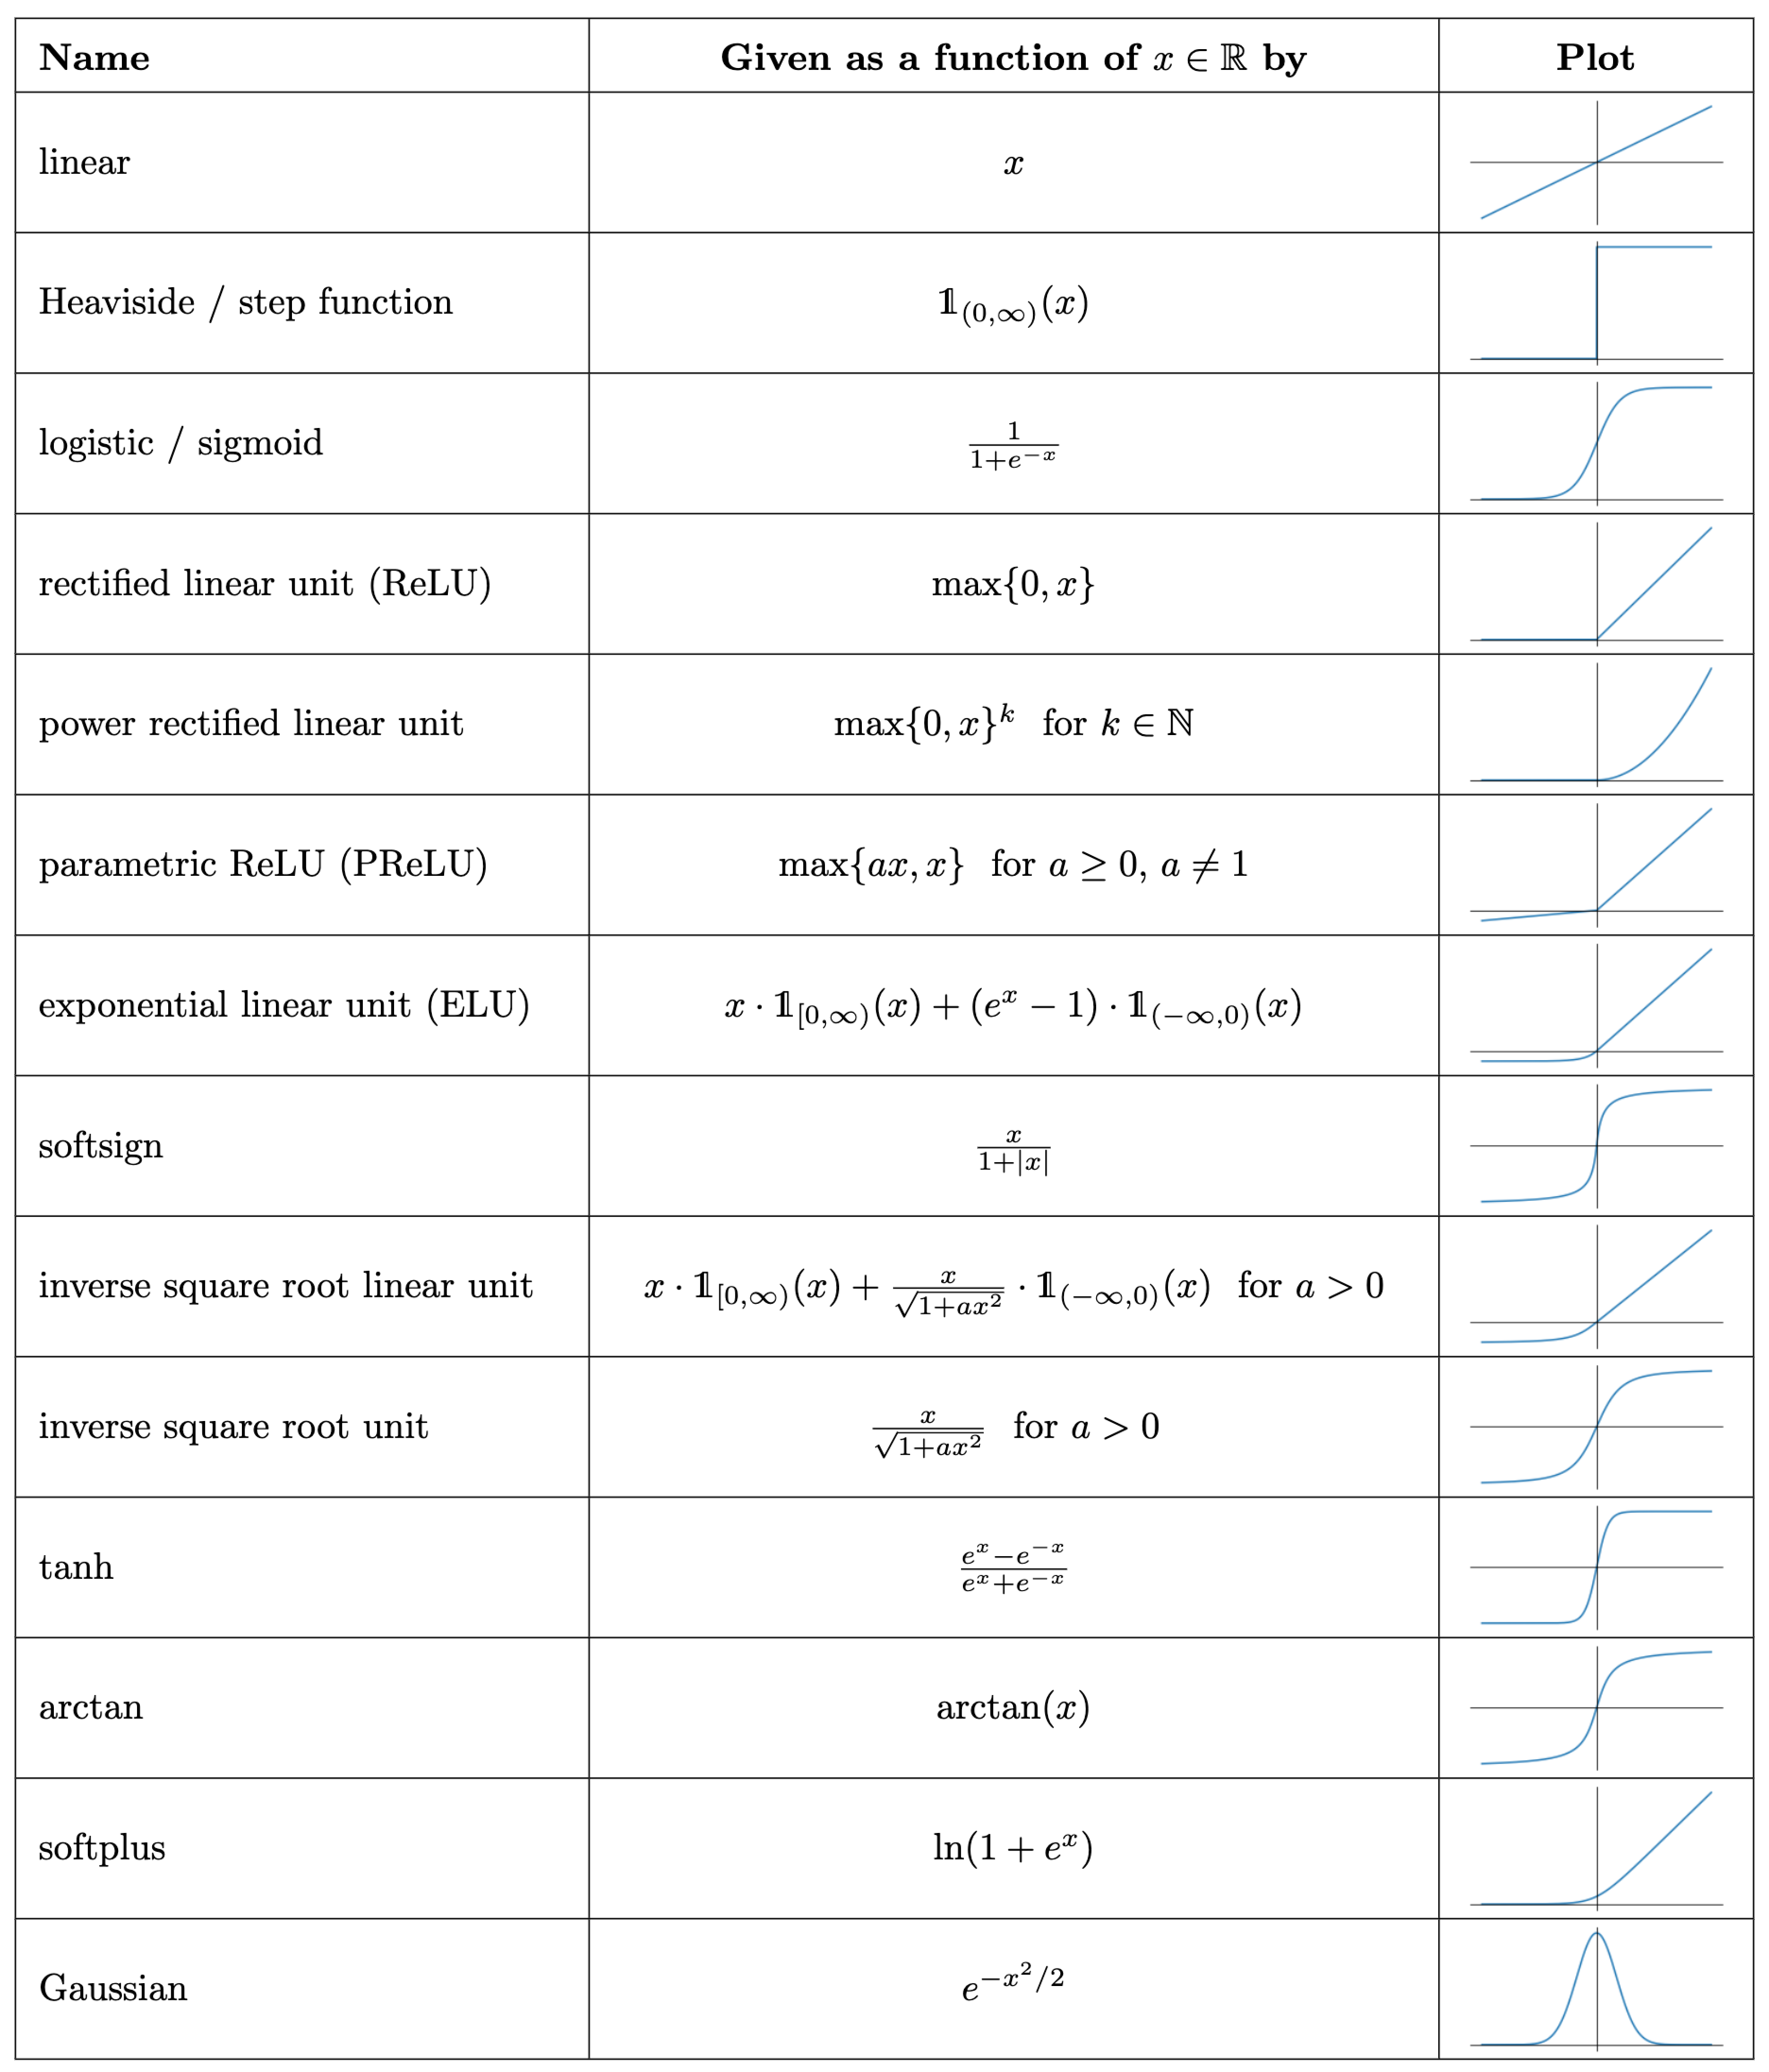
\includegraphics[width=\textwidth, height=18cm, keepaspectratio=true]{images/activation_functions.png}
    \captionof{figure}{List of commonly used activation functions, from \cite{modern_math}.}
    \label{fig:activation_functions}
\end{center}

\end{document}
